\section{Understanding the Impacts of Health Spending on Health Outcomes}\label{sec:results}
\setstretch{1.5}

The goal of this section is to understand the impacts of health spending on health outcomes. For that we present the estimates of the impacts of the EC/29 on several fiscal and health outcomes: local expenditure, infant mortality, birth outcomes, public health infrastructure, access to health care, and ambulatorial production.

\subsection{Municipalities' Fiscal Response to the EC/29}

First, we analyse municipalities' fiscal reaction to the EC/29 using data from Finbra\footnote{In section \ref{sec:data} we describe the different sources of public spending data.}. Panel A in Table \ref{table:fiscal} presents the estimates for total public revenue, and revenues by source. In general, we find no significant effect on revenues per capita (columns 1-3) and no shift in the relevance of each source for the composition of total revenue (columns 4-6). Next, Panel B, we present the effects on total public spending, public spending by type and category, for per capita figures as well as the share of total spending. The distance to the EC/29 target is only significantly associated with Health and Sanitation spending per capita\footnote{This is the only measure of Health Spending available for the period before the EC/29 was enacted. As discussed in section \ref{sec:emp}, the validation of our research design relies partially on evaluating the presence of pre-trends. Therefore we use this variable as a proxy of health spending. In the appendix we show that }. In our preferred specification (column 3), the estimate of around 300 suggests that, a municipality with a distance to the target of 10\%, increased its health spending per capita by R\$30, an increase of around 14\% relative to the baseline health spending per capita (see Table \ref{table:stats}. This distance is roughly the distance to the target of the bottom quartile of the distribution of the share of own resources spent in health in the baseline. Columns 4-6 suggest that this increase is only possible by reallocating resources from other categories of public spending. Municipalities' increase in health spending as the share of total spending was accompanied by reductions in share of resources allocated in Transport, Education and Culture, Social Assistance, and Other Categories. The last category presented the most pronounced reduction, half of the increase in the share of resources allocated to Health and Sanitation. This category includes mainly expenditures relative to the maintenance of the administrative structure.

Figures \ref{fig:6} \ref{fig:7} \ref{fig:8}

\begin{table}[h!]
\begin{footnotesize}
\begin{center}
\scalebox{0.8}{
\begin{threeparttable}[b]

  \centering
  \caption{Fiscal Reactions}
     \begin{tabular}{rrrrrr}
          &       &       &       &       &  \\
    \midrule
    \midrule
          &       & \multicolumn{1}{c}{(1)} & \multicolumn{1}{c}{(2)} & \multicolumn{1}{c}{(3)} & \multicolumn{1}{c}{(4)} \\
    \midrule
    \multicolumn{1}{p{17.645em}}{\textbf{A. Public Revenue per capita (Finbra)}} &       &       &       &       &  \\
    \multicolumn{1}{p{17.645em}}{Total Revenue} &       & \multicolumn{1}{c}{836.808} & \multicolumn{1}{c}{863.702} & \multicolumn{1}{c}{906.461} & \multicolumn{1}{c}{924.916} \\
          &       & \multicolumn{1}{c}{(1246.358)} & \multicolumn{1}{c}{(1261.693)} & \multicolumn{1}{c}{(1259.601)} & \multicolumn{1}{c}{(1261.256)} \\
          &       &       &       &       &  \\
    \midrule
    \multicolumn{1}{p{17.645em}}{\textbf{B. Public Spending per capita (Finbra)}} &       &       &       &       &  \\
    \multicolumn{1}{p{17.645em}}{Total Spending} &       & \multicolumn{1}{c}{1087.221} & \multicolumn{1}{c}{1113.132} & \multicolumn{1}{c}{1150.066} & \multicolumn{1}{c}{1116.422} \\
          &       & \multicolumn{1}{c}{(1447.687)} & \multicolumn{1}{c}{(1464.348)} & \multicolumn{1}{c}{(1462.633)} & \multicolumn{1}{c}{(1463.927)} \\
    \multicolumn{1}{p{17.645em}}{\textbf{By Type}} &       &       &       &       &  \\
    \multicolumn{1}{p{17.645em}}{Human Resources Spending} &       & \multicolumn{1}{c}{379.094} & \multicolumn{1}{c}{387.236} & \multicolumn{1}{c}{401.055} & \multicolumn{1}{c}{369.758} \\
          &       & \multicolumn{1}{c}{(467.975)} & \multicolumn{1}{c}{(473.533)} & \multicolumn{1}{c}{(473.072)} & \multicolumn{1}{c}{(473.041)} \\
    \multicolumn{1}{p{17.645em}}{Investment Spending} &       & \multicolumn{1}{c}{-3.655} & \multicolumn{1}{c}{-5.16} & \multicolumn{1}{c}{0.894} & \multicolumn{1}{c}{0.582} \\
          &       & \multicolumn{1}{c}{(60.544)} & \multicolumn{1}{c}{(61.56)} & \multicolumn{1}{c}{(60.118)} & \multicolumn{1}{c}{(60.201)} \\
    \multicolumn{1}{p{17.645em}}{Other Spending} &       & \multicolumn{1}{c}{714.17} & \multicolumn{1}{c}{734.512} & \multicolumn{1}{c}{751.919} & \multicolumn{1}{c}{750.087} \\
          &       & \multicolumn{1}{c}{(980.705)} & \multicolumn{1}{c}{(992.273)} & \multicolumn{1}{c}{(991.445)} & \multicolumn{1}{c}{(992.396)} \\
    \multicolumn{1}{p{17.645em}}{\textbf{By Category}} &       &       &       &       &  \\
    \multicolumn{1}{p{17.645em}}{Health and Sanitation Spending} &       & \multicolumn{1}{c}{301.558***} & \multicolumn{1}{c}{305.893***} & \multicolumn{1}{c}{313.09***} & \multicolumn{1}{c}{306.849***} \\
          &       & \multicolumn{1}{c}{(94.325)} & \multicolumn{1}{c}{(95.601)} & \multicolumn{1}{c}{(94.6)} & \multicolumn{1}{c}{(94.649)} \\
    \multicolumn{1}{p{17.645em}}{Transport Spending} &       & \multicolumn{1}{c}{54.117} & \multicolumn{1}{c}{56.175} & \multicolumn{1}{c}{58.192} & \multicolumn{1}{c}{59.046} \\
          &       & \multicolumn{1}{c}{(64.464)} & \multicolumn{1}{c}{(65.544)} & \multicolumn{1}{c}{(65.499)} & \multicolumn{1}{c}{(65.563)} \\
    \multicolumn{1}{p{17.645em}}{Education and Culture Spending} &       & \multicolumn{1}{c}{181.354} & \multicolumn{1}{c}{192.539} & \multicolumn{1}{c}{202.462} & \multicolumn{1}{c}{194.738} \\
          &       & \multicolumn{1}{c}{(390.341)} & \multicolumn{1}{c}{(395.815)} & \multicolumn{1}{c}{(395.515)} & \multicolumn{1}{c}{(395.841)} \\
    \multicolumn{1}{p{17.645em}}{Housing and Urban Spending} &       & \multicolumn{1}{c}{106.013} & \multicolumn{1}{c}{103.406} & \multicolumn{1}{c}{107.639} & \multicolumn{1}{c}{105.529} \\
          &       & \multicolumn{1}{c}{(151.518)} & \multicolumn{1}{c}{(153.227)} & \multicolumn{1}{c}{(152.911)} & \multicolumn{1}{c}{(153.047)} \\
    \multicolumn{1}{p{17.645em}}{Social Assistance Spending per capita} &       & \multicolumn{1}{c}{189.164} & \multicolumn{1}{c}{197.27} & \multicolumn{1}{c}{200.542} & \multicolumn{1}{c}{200.274} \\
          &       & \multicolumn{1}{c}{(250.997)} & \multicolumn{1}{c}{(254.167)} & \multicolumn{1}{c}{(254.074)} & \multicolumn{1}{c}{(254.271)} \\
    \multicolumn{1}{p{17.645em}}{Spending in Other Categories per capita} &       & \multicolumn{1}{c}{360.927} & \multicolumn{1}{c}{363.75} & \multicolumn{1}{c}{379.137} & \multicolumn{1}{c}{363.341} \\
          &       & \multicolumn{1}{c}{(667.376)} & \multicolumn{1}{c}{(675.284)} & \multicolumn{1}{c}{(674.371)} & \multicolumn{1}{c}{(674.972)} \\
          &       &       &       &       &  \\
    \midrule
    \multicolumn{1}{p{17.645em}}{\textbf{C. Public Health Spending (SIOPS)}} &       &       &       &       &  \\
    \multicolumn{1}{p{17.645em}}{Total} &       & \multicolumn{1}{c}{527.781***} & \multicolumn{1}{c}{528.862***} & \multicolumn{1}{c}{529.49***} & \multicolumn{1}{c}{528.868***} \\
          &       & \multicolumn{1}{c}{(18.128)} & \multicolumn{1}{c}{(17.841)} & \multicolumn{1}{c}{(17.472)} & \multicolumn{1}{c}{(17.45)} \\
    \multicolumn{1}{p{17.645em}}{\textbf{By Source}} &       &       &       &       &  \\
    \multicolumn{1}{p{17.645em}}{Own Resources} &       & \multicolumn{1}{c}{579.68***} & \multicolumn{1}{c}{580.296***} & \multicolumn{1}{c}{580.493***} & \multicolumn{1}{c}{580.069***} \\
          &       & \multicolumn{1}{c}{(13.917)} & \multicolumn{1}{c}{(13.696)} & \multicolumn{1}{c}{(13.392)} & \multicolumn{1}{c}{(13.402)} \\
    \multicolumn{1}{p{17.645em}}{Transfers} &       & \multicolumn{1}{c}{-53.721***} & \multicolumn{1}{c}{-53.2***} & \multicolumn{1}{c}{-52.546***} & \multicolumn{1}{c}{-52.757***} \\
          &       & \multicolumn{1}{c}{(11.257)} & \multicolumn{1}{c}{(11.147)} & \multicolumn{1}{c}{(11.114)} & \multicolumn{1}{c}{(11.099)} \\
    \multicolumn{1}{p{17.645em}}{\textbf{By Type}} &       &       &       &       &  \\
    \multicolumn{1}{p{17.645em}}{Human Resources} &       & \multicolumn{1}{c}{96.582***} & \multicolumn{1}{c}{94.588***} & \multicolumn{1}{c}{94.88***} & \multicolumn{1}{c}{92.829***} \\
          &       & \multicolumn{1}{c}{(11.183)} & \multicolumn{1}{c}{(11.1)} & \multicolumn{1}{c}{(10.98)} & \multicolumn{1}{c}{(10.895)} \\
    \multicolumn{1}{p{17.645em}}{Investiment} &       & \multicolumn{1}{c}{132.581***} & \multicolumn{1}{c}{132.998***} & \multicolumn{1}{c}{133.035***} & \multicolumn{1}{c}{133.256***} \\
          &       & \multicolumn{1}{c}{(9.637)} & \multicolumn{1}{c}{(9.665)} & \multicolumn{1}{c}{(9.649)} & \multicolumn{1}{c}{(9.654)} \\
    \multicolumn{1}{p{17.645em}}{3rd parties services} &       & \multicolumn{1}{c}{55.767***} & \multicolumn{1}{c}{54.76***} & \multicolumn{1}{c}{54.646***} & \multicolumn{1}{c}{55.06***} \\
          &       & \multicolumn{1}{c}{(11.661)} & \multicolumn{1}{c}{(11.519)} & \multicolumn{1}{c}{(11.445)} & \multicolumn{1}{c}{(11.464)} \\
    \multicolumn{1}{p{17.645em}}{Other Expenditures} &       & \multicolumn{1}{c}{246.578***} & \multicolumn{1}{c}{249.698***} & \multicolumn{1}{c}{250.095***} & \multicolumn{1}{c}{250.871***} \\
          &       & \multicolumn{1}{c}{(11.355)} & \multicolumn{1}{c}{(11.408)} & \multicolumn{1}{c}{(11.394)} & \multicolumn{1}{c}{(11.36)} \\
          &       &       &       &       &  \\
    \bottomrule
    \bottomrule
    \end{tabular}%
    
    
  \label{table:fiscal}%
  
  \begin{tablenotes}
  \scriptsize{\underline{Notes}: The number of observations is 64224 for Finbra variables and  56012 for SIOPS variables.  DiD Estimates from Equation \ref{eq:1}. Independent variable is the distance to the EC/29 target in p.p. Column 1 presents the baseline model with municipality and state-year fixed effects. Column 2 adds baseline socioeconomic controls from the Census interacted with time. Column 3 adds controls for GDP per capita and \emph{Bolsa Familia} transfers per capita. Column 4 adds fiscal controls. Covariates ommited. Standard errors in brackets are clustered in the municipality level. ∗p < 0.10, ∗ ∗ p < 0.05, ∗ ∗ ∗p < 0.01}
  \end{tablenotes}

\end{threeparttable}
}
\end{center}
\end{footnotesize}
\end{table}

\begin{figure}[h!]
    \begin{center}
    \caption{Fiscal Reactions}\label{fig:6}
    \begin{subfigure}{0.49\textwidth}
        \caption{\scriptsize Total Revenue}\label{fig:6a}
        \centering
        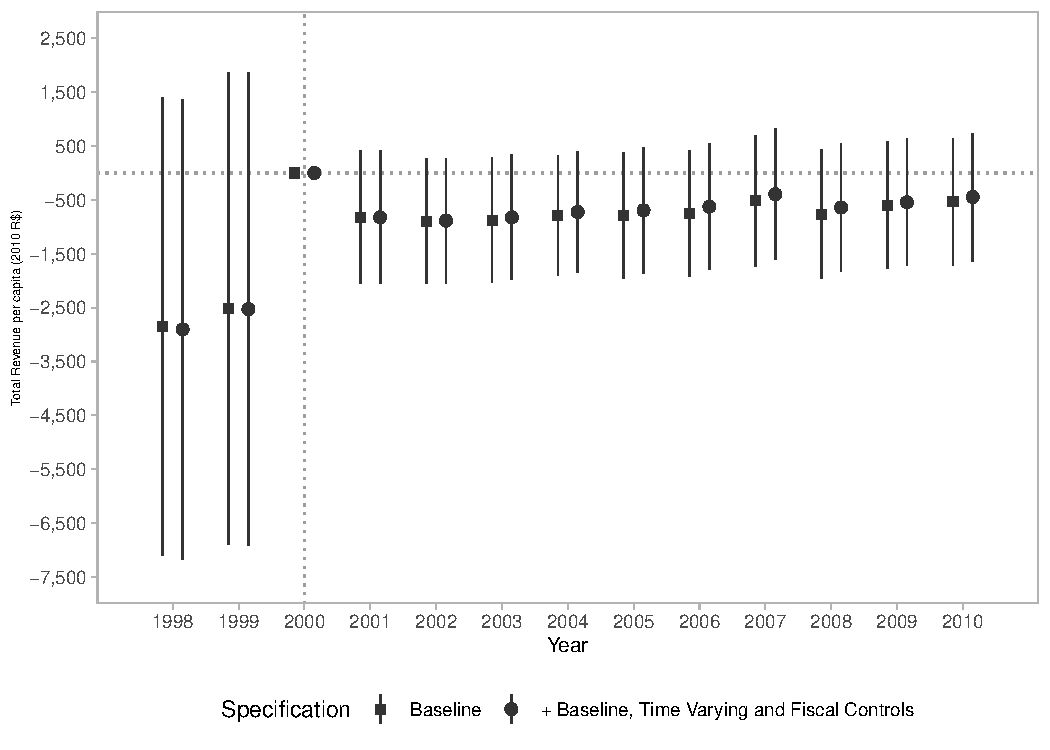
\includegraphics[width=\textwidth]{plots/finbra_reccorr_pcapita_dist_ec29_baseline_dist_ec29_baseline_6.pdf}
    \end{subfigure}
    \begin{subfigure}{0.49\textwidth}
        \centering
        \caption{\scriptsize Total Public Spending}\label{fig:6b}
        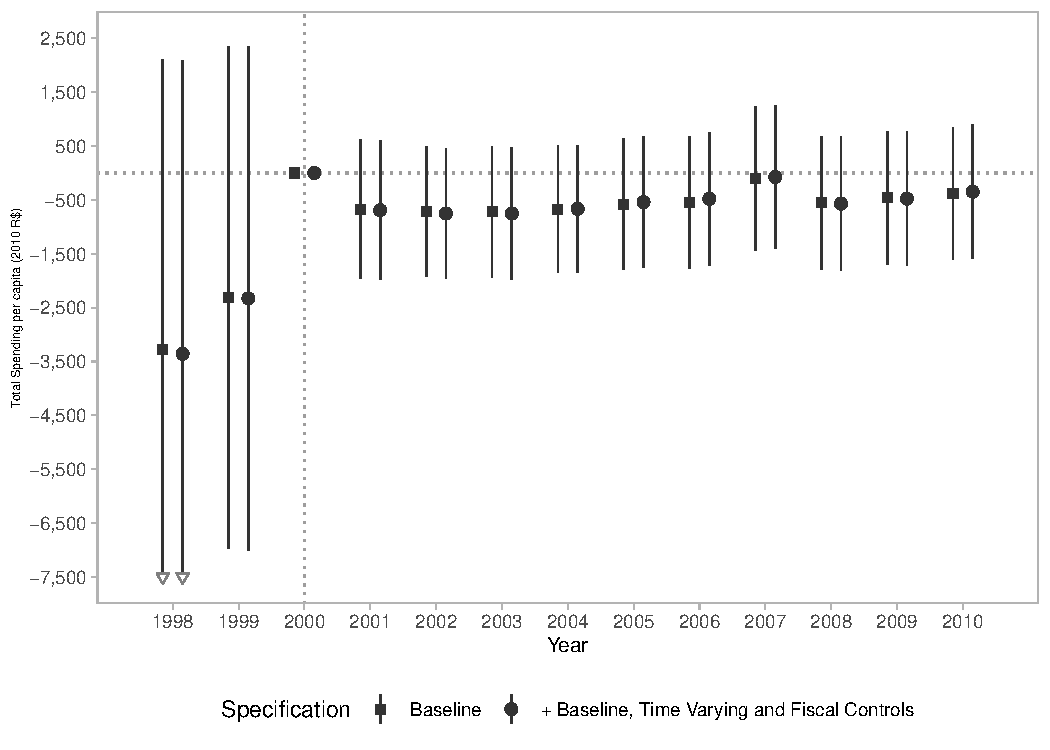
\includegraphics[width=\textwidth]{plots/finbra_desp_o_pcapita_dist_ec29_baseline_dist_ec29_baseline_6.pdf}
    \end{subfigure}
    
    \end{center}
    \scriptsize{Notes: The number of observations is 64224. DiD Estimates from Equation \ref{eq:2}. Independent variable is the distance to the EC/29 target in p.p. Square dots represent the baseline model with municipality and state-year fixed effects. Round dots represent fully saturated specification (Column 4 in regression Tables). Lines represent 95\% confidence intervals. Arrows, when present, indicate confidence intervals out of the plot bounds. Standard errors are clustered in the municipality level.}
    
\end{figure}

\begin{figure}[h!]
    \begin{center}
    \caption{Effects Public Spending per capita - By Type}\label{fig:7}
    \begin{subfigure}{0.32\textwidth}
        \centering
        \caption{\scriptsize Human Resources}\label{fig:7a}
        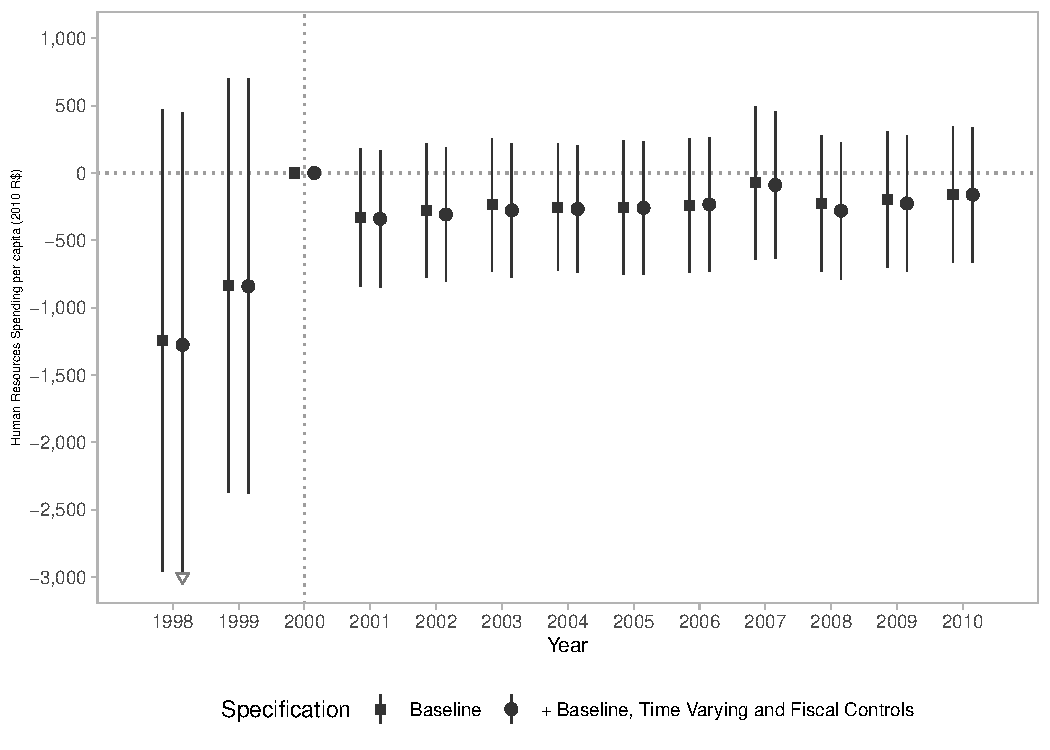
\includegraphics[width=\textwidth]{plots/finbra_desp_pessoal_pcapita_dist_ec29_baseline_dist_ec29_baseline_7.pdf}
    \end{subfigure}
    \begin{subfigure}{0.32\textwidth}
        \centering
        \caption{\scriptsize Investments}\label{fig:7b}
        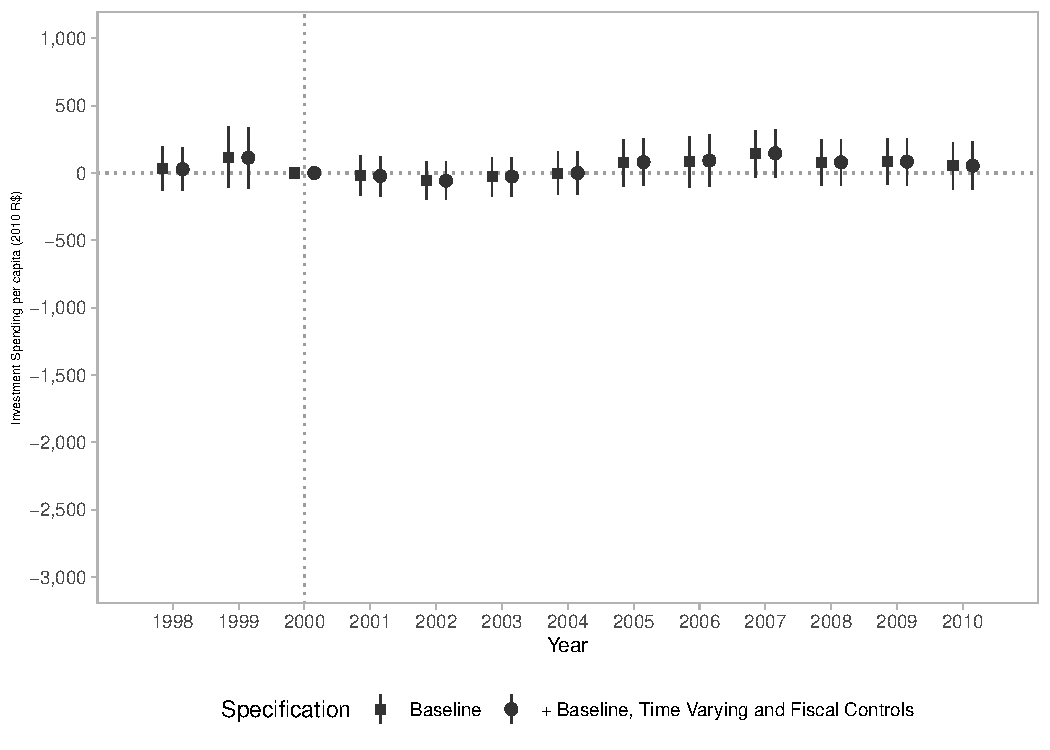
\includegraphics[width=\textwidth]{plots/finbra_desp_investimento_pcapita_dist_ec29_baseline_dist_ec29_baseline_7.pdf}
    \end{subfigure}
    \begin{subfigure}{0.32\textwidth}
        \centering
        \caption{\scriptsize Other}\label{fig:7c}
        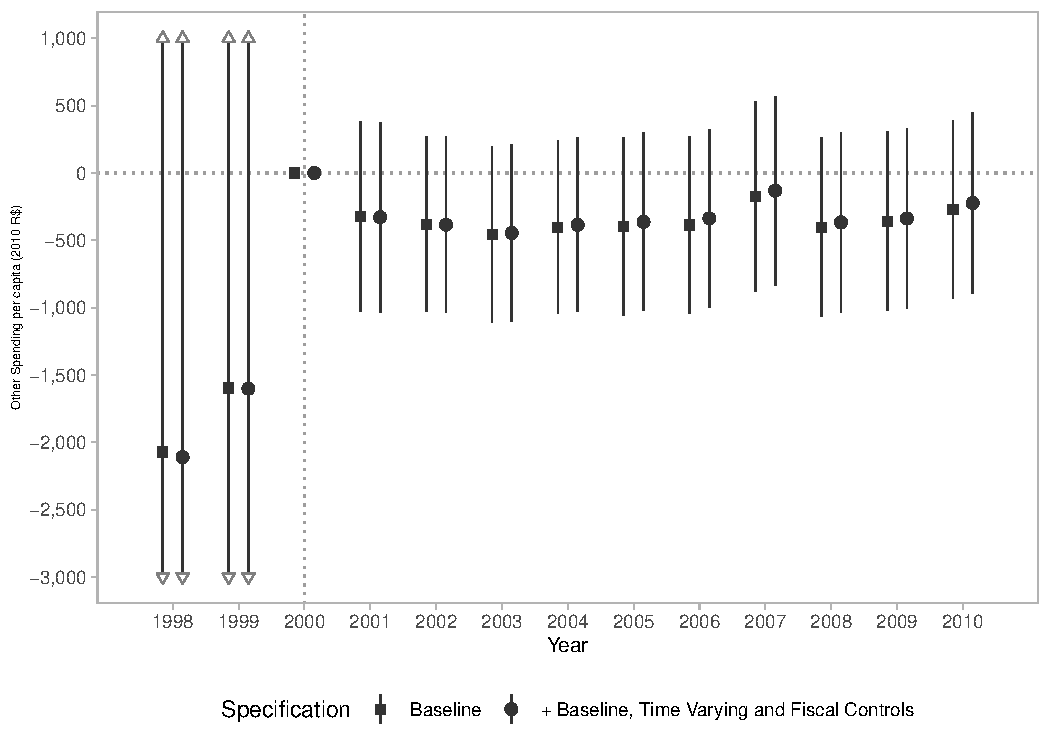
\includegraphics[width=\textwidth]{plots/finbra_desp_outros_nature_pcapita_dist_ec29_baseline_dist_ec29_baseline_7.pdf}
    \end{subfigure}
    
    \end{center}
    \scriptsize{Notes: The number of observations is 64224. DiD Estimates from Equation \ref{eq:2}. Independent variable is the distance to the EC/29 target in p.p. Square dots represent the baseline model with municipality and state-year fixed effects. Round dots represent fully saturated specification (Column 4 in regression Tables). Lines represent 95\% confidence intervals. Arrows, when present, indicate confidence intervals out of the plot bounds. Standard errors are clustered in the municipality level.}
    
\end{figure}

\begin{figure}[h!]
    \begin{center}
    \caption{Effects on Public Spending per capita - By Category}\label{fig:8}
    \begin{subfigure}{0.48\textwidth}
        \caption{\scriptsize Health and Sanitation}\label{fig:8a}
        \centering
        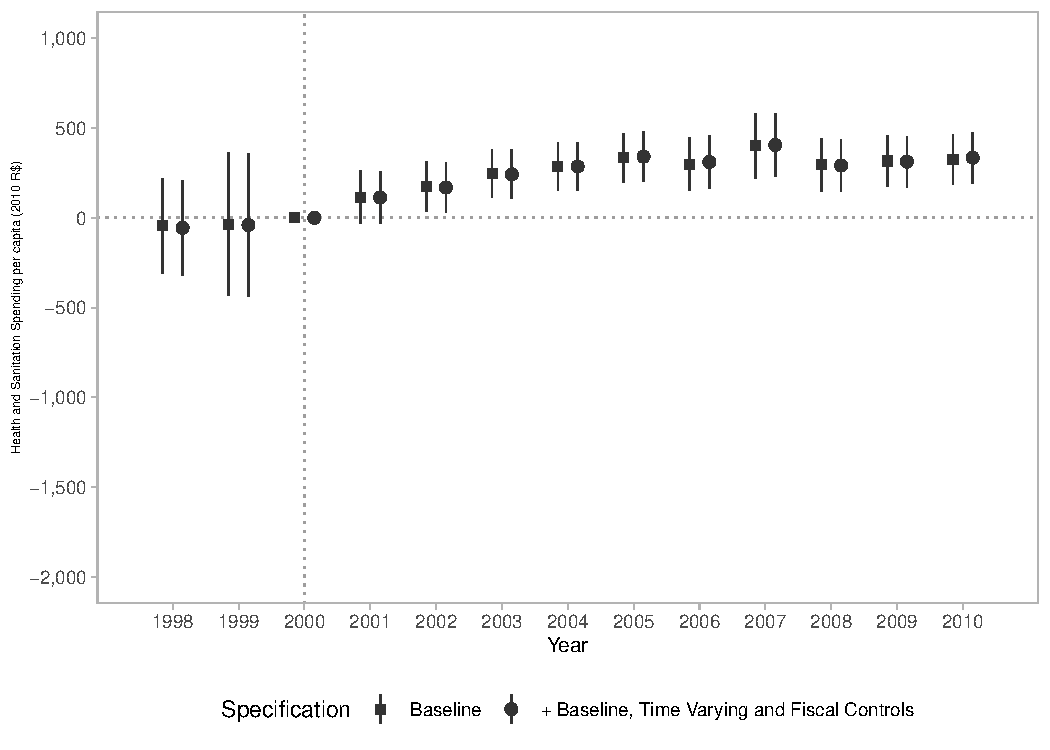
\includegraphics[width=\textwidth]{plots/finbra_desp_saude_san_pcapita_dist_ec29_baseline_dist_ec29_baseline_8.pdf}
    \end{subfigure}
    \begin{subfigure}{0.48\textwidth}
        \centering
        \caption{\scriptsize Education and Culture}\label{fig:8b}
        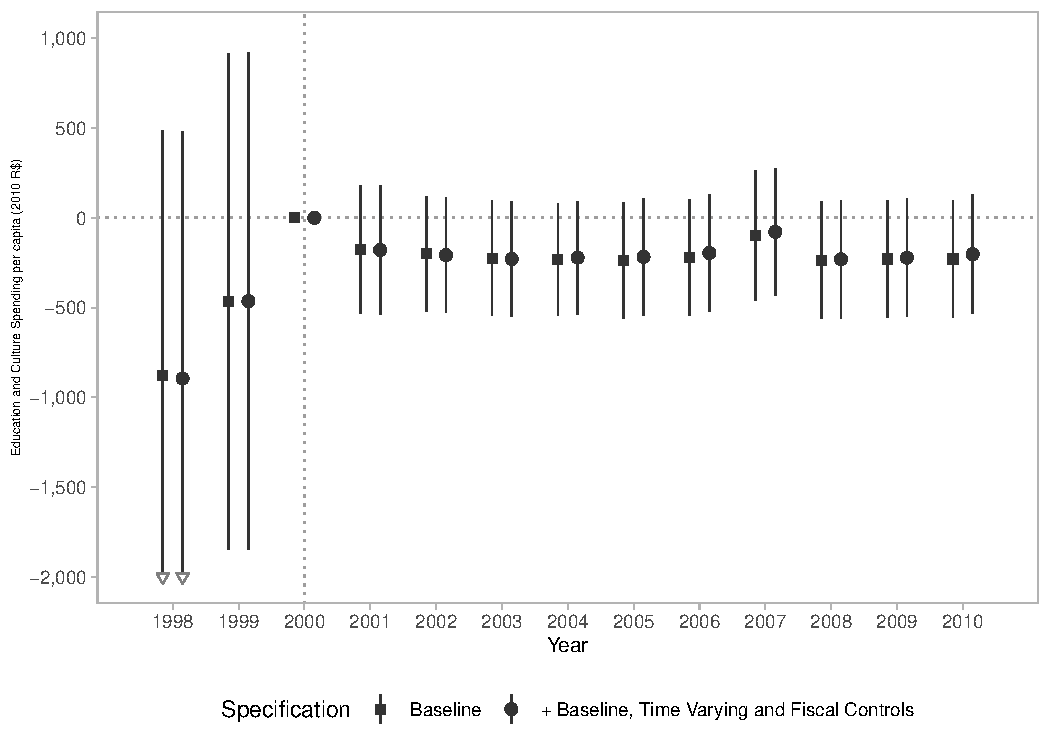
\includegraphics[width=\textwidth]{plots/finbra_desp_educ_cultura_pcapita_dist_ec29_baseline_dist_ec29_baseline_8.pdf}
    \end{subfigure}
    \begin{subfigure}{0.48\textwidth}
        \centering
        \caption{\scriptsize Social Assistance}\label{fig:8c}
        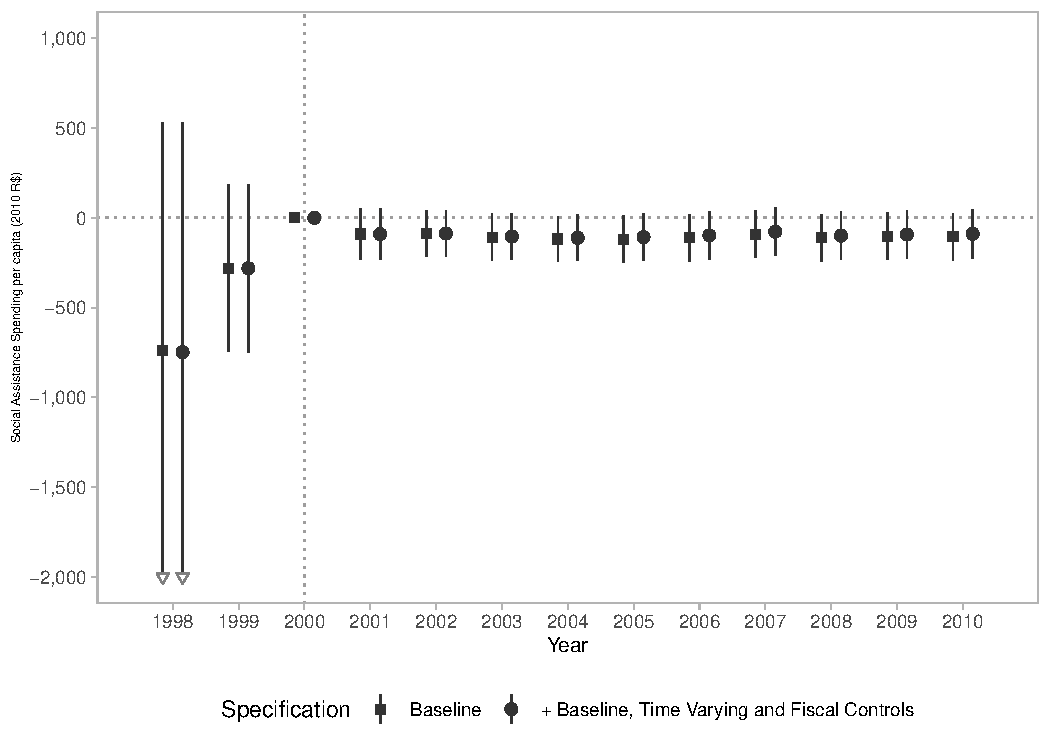
\includegraphics[width=\textwidth]{plots/finbra_desp_assist_prev_pcapita_dist_ec29_baseline_dist_ec29_baseline_8.pdf}
    \end{subfigure}
    \begin{subfigure}{0.48\textwidth}
        \centering
        \caption{\scriptsize Transport}\label{fig:8d}
        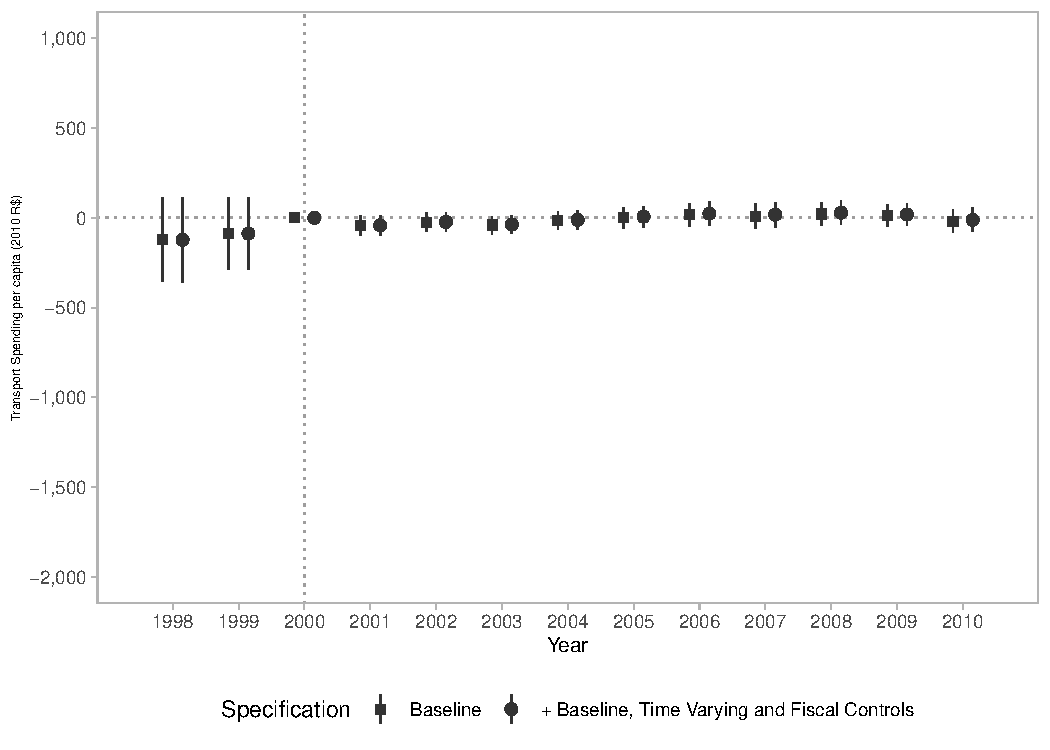
\includegraphics[width=\textwidth]{plots/finbra_desp_transporte_pcapita_dist_ec29_baseline_dist_ec29_baseline_8.pdf}
    \end{subfigure}
    \begin{subfigure}{0.48\textwidth}
        \centering
        \caption{\scriptsize Housing and Urban}\label{fig:8e}
        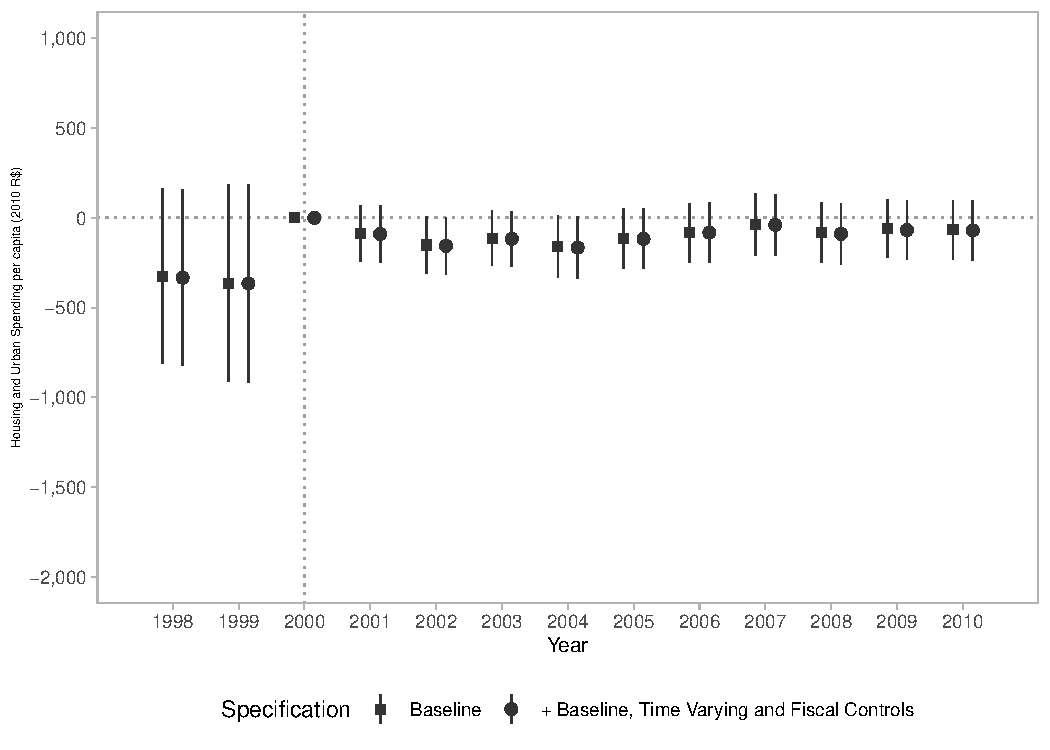
\includegraphics[width=\textwidth]{plots/finbra_desp_hab_urb_pcapita_dist_ec29_baseline_dist_ec29_baseline_8.pdf}
    \end{subfigure}
    \begin{subfigure}{0.48\textwidth}
        \centering
        \caption{\scriptsize Spending in Other Categories}\label{fig:8f}
        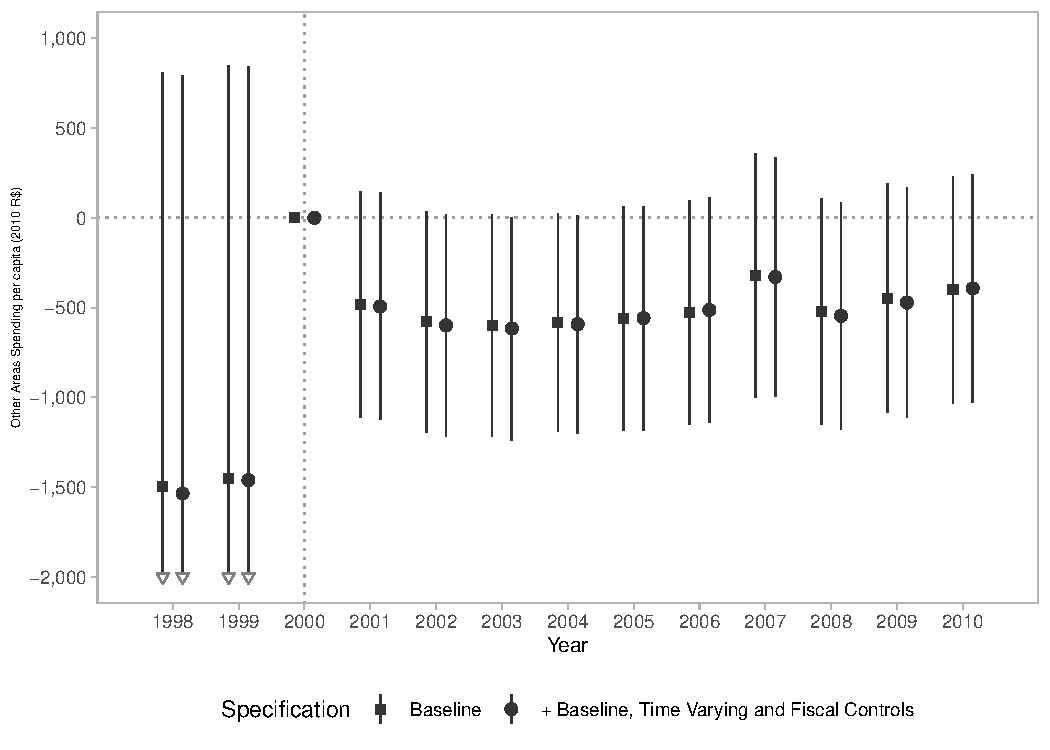
\includegraphics[width=\textwidth]{plots/finbra_desp_outros_area_pcapita_dist_ec29_baseline_dist_ec29_baseline_8.pdf}
    \end{subfigure}
    
    \end{center}
    \scriptsize{Notes: The number of observations is 64224. DiD Estimates from Equation \ref{eq:2}. Independent variable is the distance to the EC/29 target in p.p. Square dots represent the baseline model with municipality and state-year fixed effects. Round dots represent fully saturated specification (Column 4 in regression Tables). Lines represent 95\% confidence intervals. Arrows, when present, indicate confidence intervals out of the plot bounds. Standard errors are clustered in the municipality level.}
    
\end{figure}

Though SIOPS data is only available from 2000 on, it allow us to analyse the sources of spending and the types of spending within total public health spending. Panel C in Table \ref{table:fiscal} presents the results for these variables. These results should be taken with parsimony, as these regressions do not include data for pre-treatment periods. Our estimations suggests an effect of R\$ 528 for total Health Spending per capita. A distance of 10\% to the target represents a 27\% increase relative to the baseline, almost twice the effect on Health and Sanitation per capita. It makes sense that a variable that only includes health spending presents a higher effect, as our source of variation is expected to move health spending only. Additionally, as presented in Panel C this effect comes almost entirely from increases in spending from own resources, a five fold increase relative to own resource spending in the baseline. All types of health spending were responsible for this increase in total health spending, but the increase in investment is the noteworthy, specially in relative terms. A distance of 10\% is associated with a 90\% increase in health investments. Baseline statistics show very little resources allocated in investments within total public health spending, the great majority of resources were allocated in human resources and in other administrative expenses. Considering the importance of capital investments to the supply of medical resources and the quality of medical services, and the little amount of investments in the baseline, an effect of this size is really relevant.

[DYNAMIC EFFECTS]

Figures \ref{fig:9} \ref{fig:10}

\begin{figure}[h!]
    \begin{center}
    \caption{Effects on Public Health Spending per capita}\label{fig:9}
    \begin{subfigure}{0.48\textwidth}
        \caption{\scriptsize Health and Sanitation (Finbra)}\label{fig:9a}
        \centering
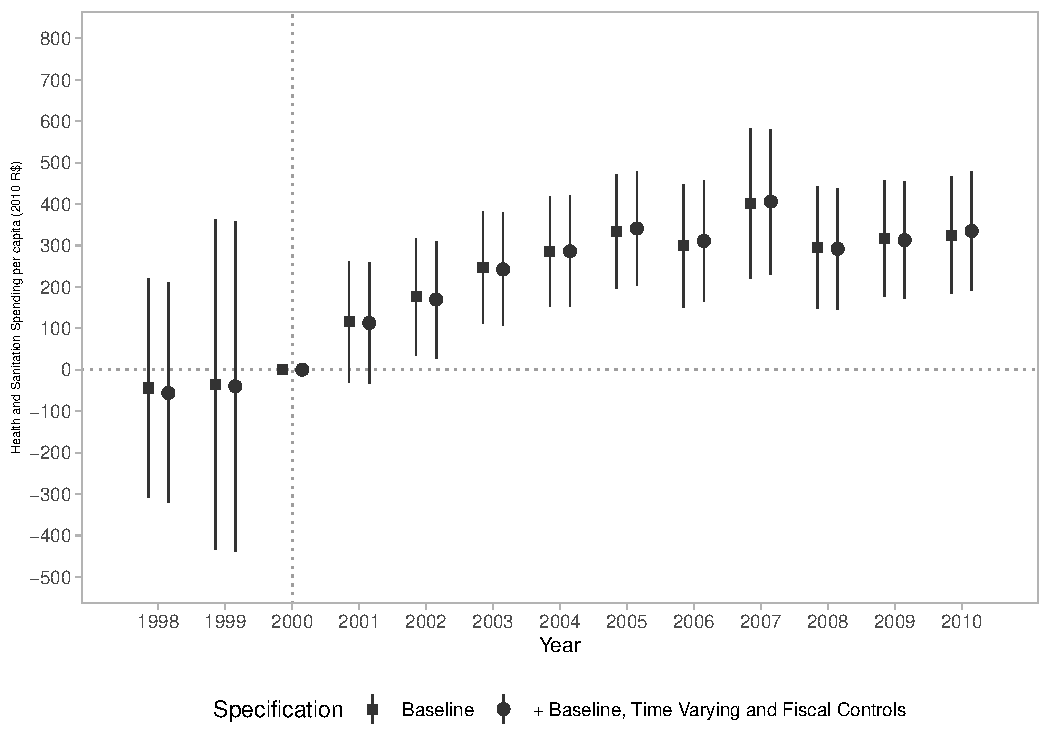
\includegraphics[width=\textwidth]{plots/finbra_desp_saude_san_pcapita_dist_ec29_baseline_dist_ec29_baseline_9.pdf}
    \end{subfigure}
    \begin{subfigure}{0.48\textwidth}
        \centering
        \caption{\scriptsize Total Health Spending (SIOPS)}\label{fig:9b}
        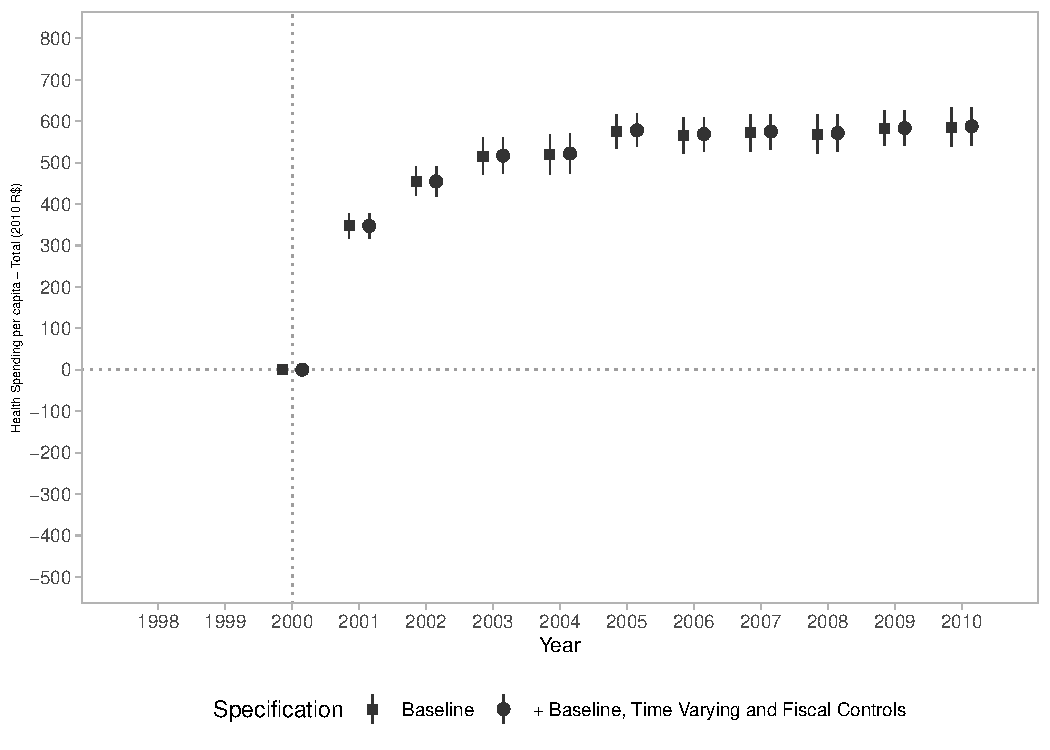
\includegraphics[width=\textwidth]{plots/siops_despsaude_pcapita_dist_ec29_baseline_dist_ec29_baseline_9.pdf}
    \end{subfigure}
    \begin{subfigure}{0.48\textwidth}
        \centering
        \caption{\scriptsize Health Spending - Own Resources (SIOPS)}\label{fig:9c}
        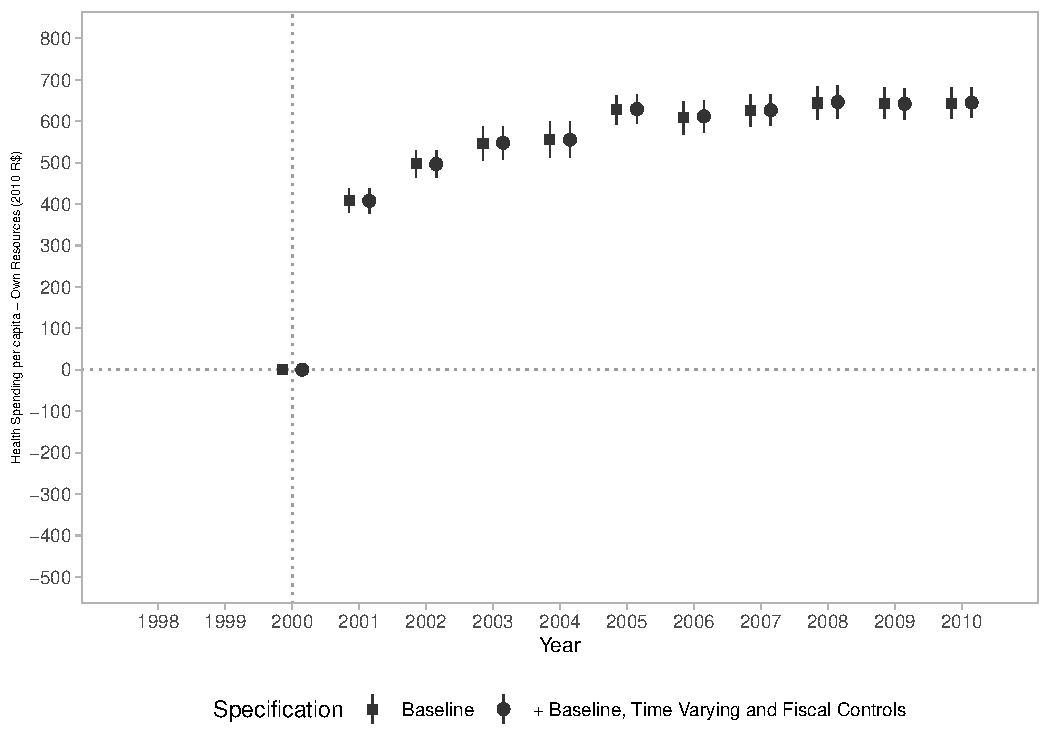
\includegraphics[width=\textwidth]{plots/siops_desprecpropriosaude_pcapita_dist_ec29_baseline_dist_ec29_baseline_9.pdf}
    \end{subfigure}
    \begin{subfigure}{0.48\textwidth}
        \centering
        \caption{\scriptsize Health Spending  - Transfers (SIOPS)}\label{fig:9d}
        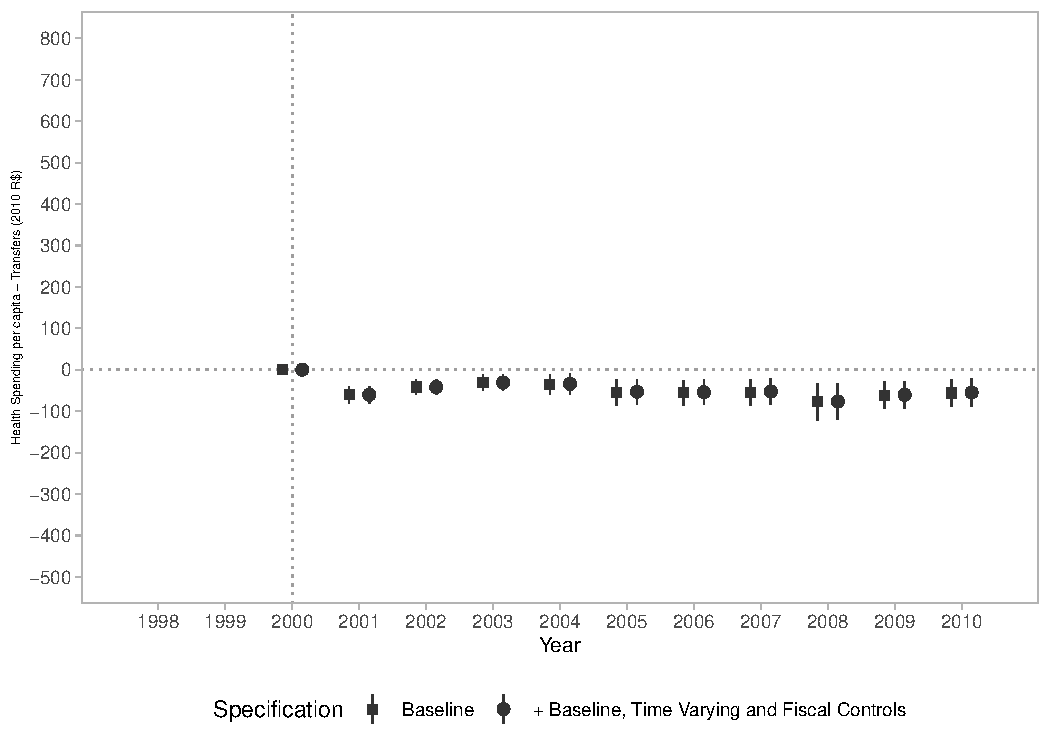
\includegraphics[width=\textwidth]{plots/siops_despexrecproprio_pcapita_dist_ec29_baseline_dist_ec29_baseline_9.pdf}
    \end{subfigure}
    
    \end{center}
    
\end{figure}

\begin{figure}[h!]
    \begin{center}
    \caption{Effects on Public Health Spending per capita - By Type}\label{fig:10}
    \begin{subfigure}{0.48\textwidth}
        \centering
        \caption{\scriptsize Human Resources}\label{fig:10a}
        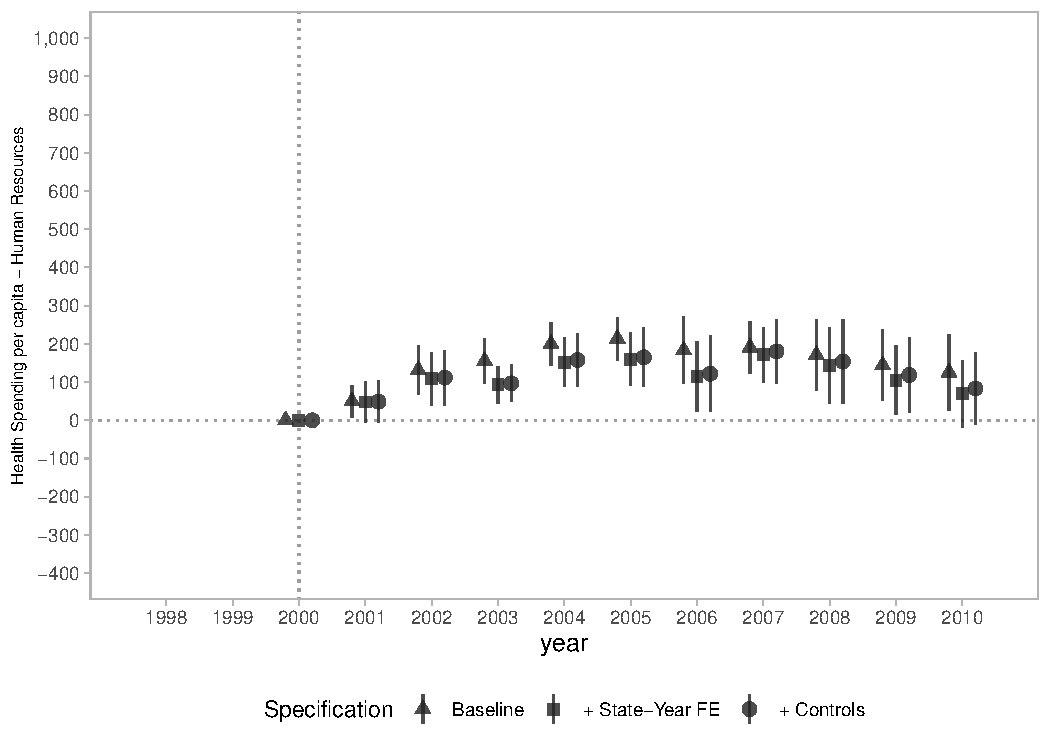
\includegraphics[width=\textwidth]{plots/spending/siops_desppessoal_pcapita_dist_ec29_baseline_dist_ec29_baseline_full.pdf}
    \end{subfigure}
    \begin{subfigure}{0.48\textwidth}
        \centering
        \caption{\scriptsize Investiment}\label{fig:10b}
        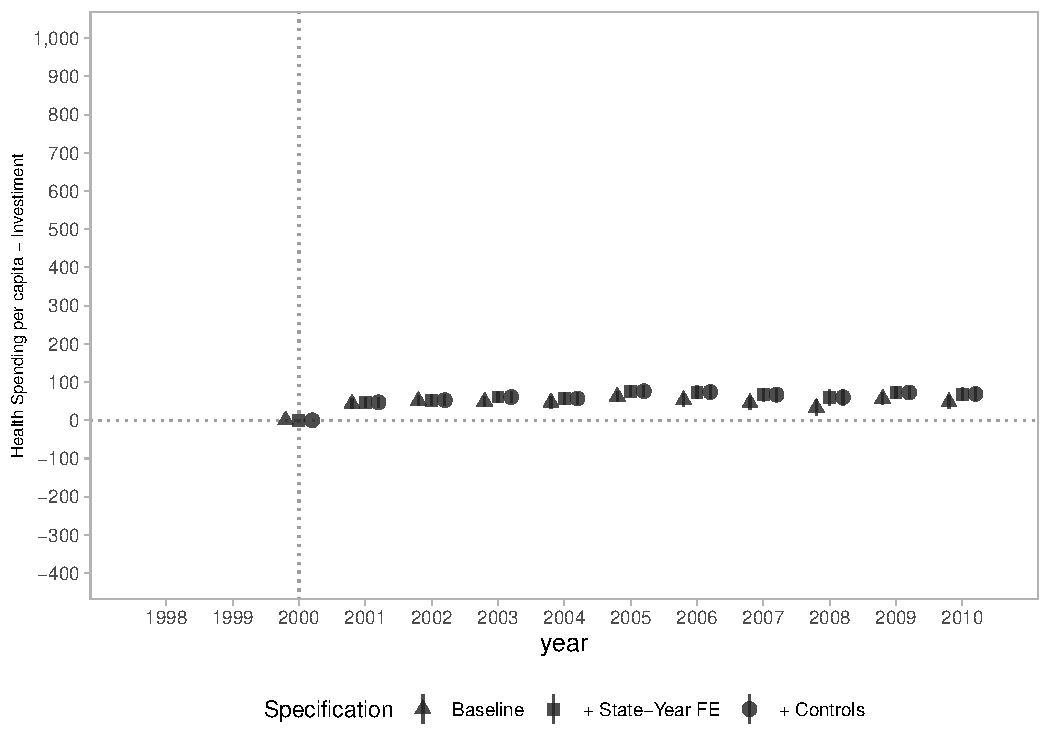
\includegraphics[width=\textwidth]{plots/spending/siops_despinvest_pcapita_dist_ec29_baseline_dist_ec29_baseline_full.pdf}
    \end{subfigure}
    \begin{subfigure}{0.48\textwidth}
        \centering
        \caption{\scriptsize 3rd parties services}\label{fig:10c}
        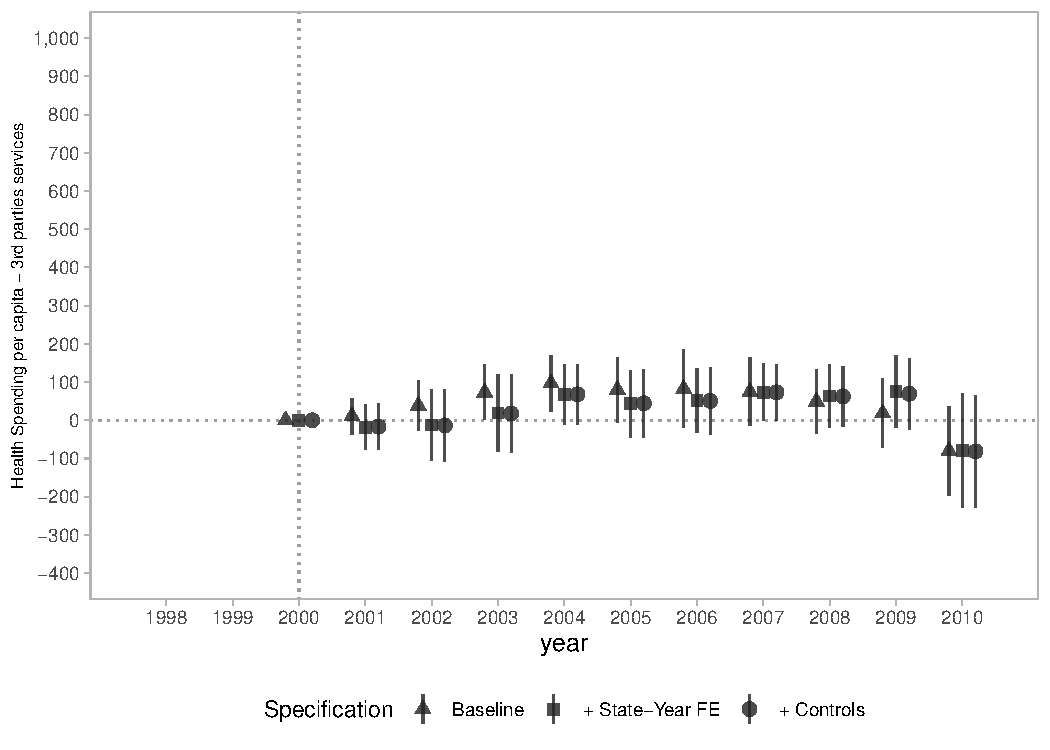
\includegraphics[width=\textwidth]{plots/spending/siops_despservicoster_pcapita_dist_ec29_baseline_dist_ec29_baseline_full.pdf}
    \end{subfigure}
    \begin{subfigure}{0.48\textwidth}
        \centering
        \caption{\scriptsize Other Expenditures}\label{fig:10d}
        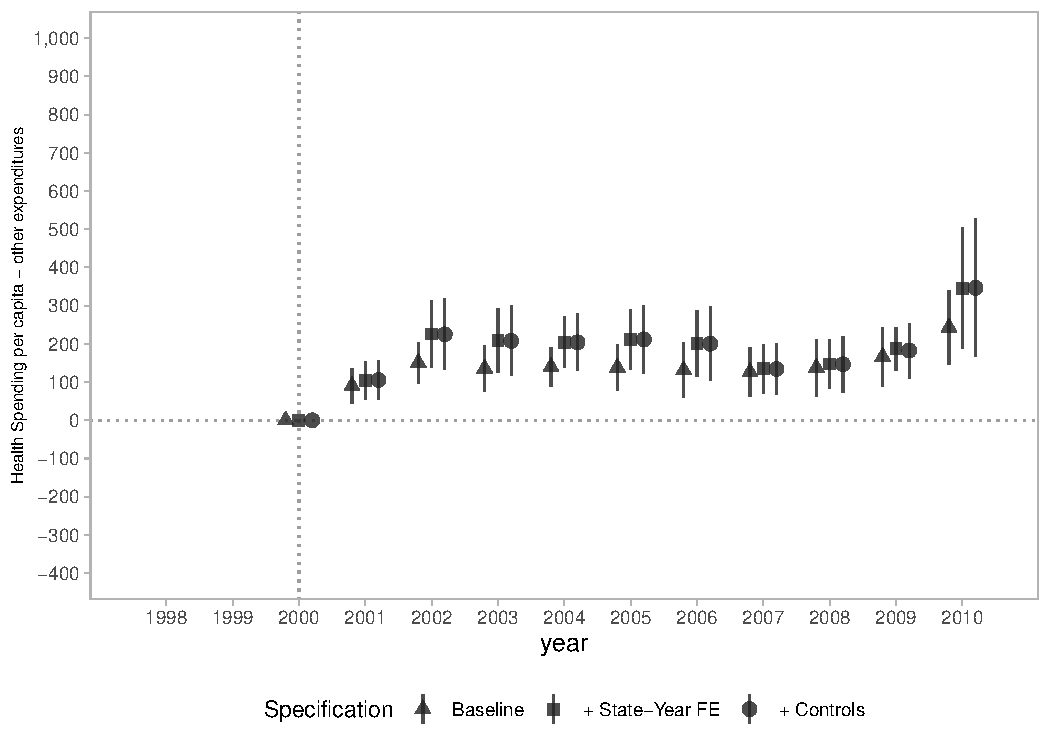
\includegraphics[width=\textwidth]{plots/spending/siops_despoutros_pcapita_dist_ec29_baseline_dist_ec29_baseline_full.pdf}
    \end{subfigure}
    
    \end{center}
    
\end{figure}


\subsection{Effects on Health Inputs}

In this subsection we aim to explore the pathways that mediate the relationship between health spending and health outcomes. For that, we explore the impacts of the EC/29 on several health inputs: access to public health services, health infrastructure, and ambulatorial production.

Table present the estimates for several health infrastructure proxies. For the period of analysis there is no direct health infrastructure data available. Using the SIA data, we are able, for each year, to count the number of facilities with ambulatorial services, in general, and classified by the type of service and type of professional associated with the service. 

Table \ref{table:infra}, Figures \ref{fig:11} \ref{fig:12} \ref{fig:13}

\begin{table}[H]
\begin{footnotesize}
\begin{center}
\scalebox{0.65}{
\begin{threeparttable}[b]

  \centering
  \caption{Primary Care Coverage, Health Infrastructure and Human Resources}
     \begin{tabular}{rrcccr}
          &       &       &       &       &  \\
    \midrule
    \midrule
          &       & \multicolumn{4}{c}{Distance to EC9 target} \\
\cmidrule{3-6}          &       & (1)   & (2)   & (3)   & \multicolumn{1}{c}{(4)} \\
    \midrule
    \multicolumn{1}{p{23.645em}}{\textbf{A. Primary Care Coverage -  Extensive Margin}} &       &       &       &       &  \\
    \multicolumn{1}{l}{\multirow{2}[0]{*}{Population covered (share) by Community Health Agents}} &       & 0.25*** & 0.245*** & 0.245*** & \multicolumn{1}{c}{0.245***} \\
          &       & (0.056) & (0.055) & (0.055) & \multicolumn{1}{c}{(0.055)} \\
    \multicolumn{1}{l}{\multirow{2}[0]{*}{Population covered (share) by Family Health Agents}} &       & 0.187*** & 0.197*** & 0.201*** & \multicolumn{1}{c}{0.2***} \\
          &       & (0.059) & (0.058) & (0.058) & \multicolumn{1}{c}{(0.058)} \\
          &       &       &       &       &  \\
    \midrule
    \multicolumn{1}{p{23.645em}}{\textbf{B. Primary Care Coverage -  Intensive Margin}} &       &       &       &       &  \\
    \multicolumn{1}{l}{\multirow{2}[0]{*}{N. of People Visited by Primary Care Agents (per capita)}} &       & 0.294*** & 0.287*** & 0.298*** & \multicolumn{1}{c}{0.297***} \\
          &       & (0.101) & (0.097) & (0.097) & \multicolumn{1}{c}{(0.097)} \\
    \multicolumn{1}{l}{\multirow{2}[0]{*}{N. of People Visited by Community Health Agents (per capita)}} &       & -0.028 & -0.025 & -0.026 & \multicolumn{1}{c}{-0.026} \\
          &       & (0.053) & (0.053) & (0.053) & \multicolumn{1}{c}{(0.053)} \\
    \multicolumn{1}{l}{\multirow{2}[0]{*}{N. of People Visited by Family Health Agents (per capita)}} &       & 0.321*** & 0.311*** & 0.323*** & \multicolumn{1}{c}{0.322***} \\
          &       & (0.098) & (0.093) & (0.093) & \multicolumn{1}{c}{(0.093)} \\
    \multicolumn{1}{l}{\multirow{2}[0]{*}{N. of Household Visits (per capita)}} &       & 1.059*** & 1.057*** & 1.085*** & \multicolumn{1}{c}{1.085***} \\
          &       & (0.325) & (0.325) & (0.324) & \multicolumn{1}{c}{(0.324)} \\
    \multicolumn{1}{l}{\multirow{2}[0]{*}{N. of Household Visits by Community Health Agents (per capita)}} &       & 0.396 & 0.375 & 0.368 & \multicolumn{1}{c}{0.37} \\
          &       & (0.277) & (0.279) & (0.279) & \multicolumn{1}{c}{(0.278)} \\
    \multicolumn{1}{l}{\multirow{2}[0]{*}{N. of Household Visits by Family Health Agents (per capita)}} &       & 0.653** & 0.676*** & 0.711*** & \multicolumn{1}{c}{0.71***} \\
          &       & (0.256) & (0.247) & (0.246) & \multicolumn{1}{c}{(0.246)} \\
    \multicolumn{1}{l}{\multirow{2}[0]{*}{N. of Appointments (per capita)}} &       & 0.181* & 0.181* & 0.186* & \multicolumn{1}{c}{0.187*} \\
          &       & (0.108) & (0.108) & (0.109) & \multicolumn{1}{c}{(0.109)} \\
    \multicolumn{1}{l}{\multirow{2}[0]{*}{N. of Appointments from Community Health Program (per capita)}} &       & -0.015 & -0.013 & -0.013 & \multicolumn{1}{c}{-0.013} \\
          &       & (0.02) & (0.021) & (0.021) & \multicolumn{1}{c}{(0.021)} \\
    \multicolumn{1}{l}{\multirow{2}[0]{*}{N. of Appointments from Family Health Program (per capita)}} &       & 0.192* & 0.188* & 0.193* & \multicolumn{1}{c}{0.194*} \\
          &       & (0.108) & (0.107) & (0.108) & \multicolumn{1}{c}{(0.108)} \\
          &       &       &       &       &  \\
    \midrule
    \multicolumn{1}{p{23.645em}}{\textbf{C. Number of Health Facilities (per capita * 1000) with}} &       &       &       &       &  \\
    \multicolumn{1}{l}{\multirow{2}[0]{*}{Ambulatory Service}} &       & -0.094** & -0.085** & -0.08* & \multicolumn{1}{c}{ -0.08* } \\
          &       & (0.042) & (0.043) & (0.042) & \multicolumn{1}{c}{ (0.042) } \\
    \multicolumn{1}{l}{\multirow{2}[0]{*}{Ambulatory Service and PSF Teams}} &       & 0.061** & 0.059** & 0.063** & \multicolumn{1}{c}{ 0.063** } \\
          &       & (0.029) & (0.028) & (0.028) & \multicolumn{1}{c}{ (0.028) } \\
    \multicolumn{1}{l}{\multirow{2}[0]{*}{Ambulatory Service and ACS Teams}} &       & 0.046 & 0.052 & 0.056* & \multicolumn{1}{c}{ 0.056* } \\
          &       & (0.033) & (0.032) & (0.032) & \multicolumn{1}{c}{ (0.032) } \\
    \multicolumn{1}{l}{\multirow{2}[0]{*}{Ambulatory Service and Community Doctors}} &       & 0.054* & 0.056* & 0.061** & \multicolumn{1}{c}{ 0.061** } \\
          &       & (0.032) & (0.031) & (0.031) & \multicolumn{1}{c}{ (0.031) } \\
    \multicolumn{1}{l}{\multirow{2}[0]{*}{Ambulatory Service and PSF Doctors}} &       & 0.047 & 0.051* & 0.056* & \multicolumn{1}{c}{ 0.056* } \\
          &       & (0.032) & (0.03) & (0.03) & \multicolumn{1}{c}{ (0.03) } \\
    \multicolumn{1}{l}{\multirow{2}[0]{*}{Ambulatory Service and PSF Nurses}} &       & 0.033* & 0.032 & 0.034* & \multicolumn{1}{c}{ 0.034* } \\
          &       & (0.02) & (0.02) & (0.02) & \multicolumn{1}{c}{ (0.02) } \\
    \multicolumn{1}{l}{\multirow{2}[0]{*}{Ambulatory Service and PSF Nursing Assistants}} &       & 0.061** & 0.066** & 0.07** & \multicolumn{1}{c}{ 0.07** } \\
          &       & (0.031) & (0.03) & (0.029) & \multicolumn{1}{c}{ (0.029) } \\
    \multicolumn{1}{l}{\multirow{2}[0]{*}{Ambulatory Service and ACS Nurses}} &       & 0.02  & 0.023 & 0.028 & \multicolumn{1}{c}{ 0.028 } \\
          &       & (0.03) & (0.029) & (0.029) & \multicolumn{1}{c}{ (0.029) } \\
          &       &       &       &       &  \\
    \midrule
    \multicolumn{1}{p{23.645em}}{\textbf{D. Hospital and Beds}} &       &       &       &       &  \\
    \multicolumn{1}{l}{\multirow{2}[0]{*}{N. of Hospital Beds (per capita * 1000)}} &       & -0.933** & -0.803** & -0.779** & \multicolumn{1}{c}{ -0.78** } \\
          &       & (0.373) & (0.373) & (0.372) & \multicolumn{1}{c}{ (0.372) } \\
    \multicolumn{1}{l}{\multirow{2}[0]{*}{Presence of Hospital}} &       & -0.11*** & -0.082** & -0.082** & \multicolumn{1}{c}{ -0.082** } \\
          &       & (0.041) & (0.039) & (0.039) & \multicolumn{1}{c}{ (0.039) } \\
          &       &       &       &       &  \\
    \midrule
    \midrule
          &       &       &       &       &  \\
    \end{tabular}%
    
    
  \label{table:infra}%

\end{threeparttable}
}
\end{center}
\end{footnotesize}
\end{table}

\begin{figure}[h!]
    \begin{center}
    \caption{Effects on Primary Care Coverage - Extensive Margin}\label{fig:11}
    \begin{subfigure}{0.48\textwidth}
        \centering
        \caption{\scriptsize Population Covered by Community Health Agents}\label{fig:11a}
        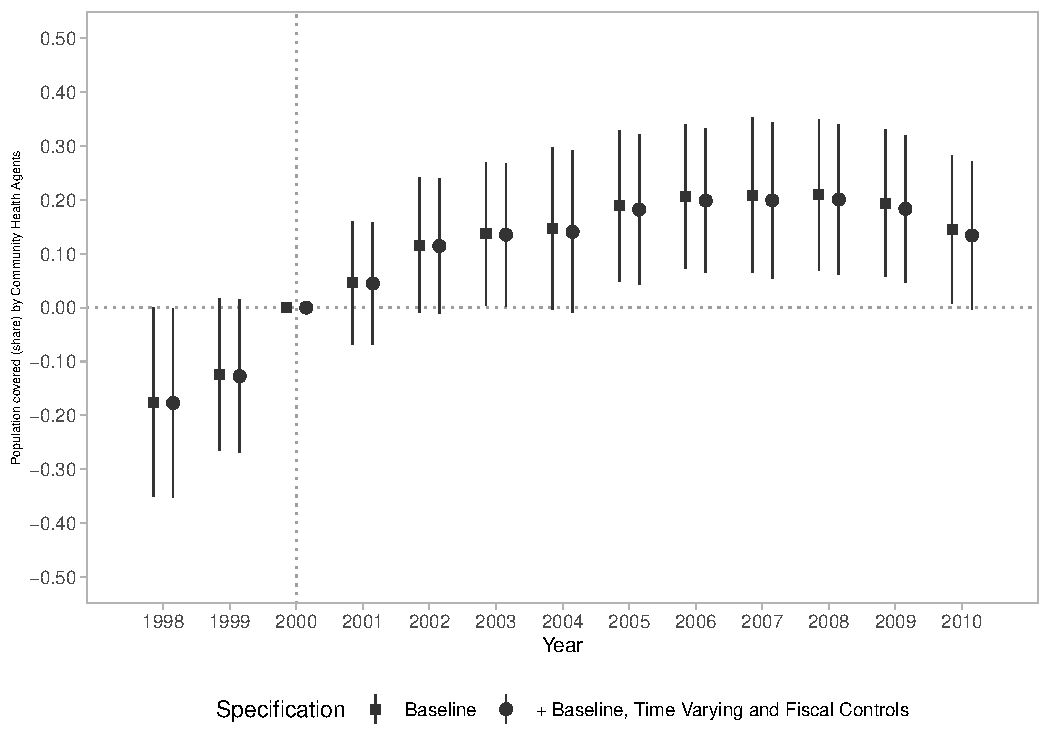
\includegraphics[width=\textwidth]{plots/ACS_popprop_dist_ec29_baseline_dist_ec29_baseline_11.pdf}
    \end{subfigure}
    \begin{subfigure}{0.48\textwidth}
        \centering
        \caption{\scriptsize Population Covered by Family Health Agents}\label{fig:1b}
        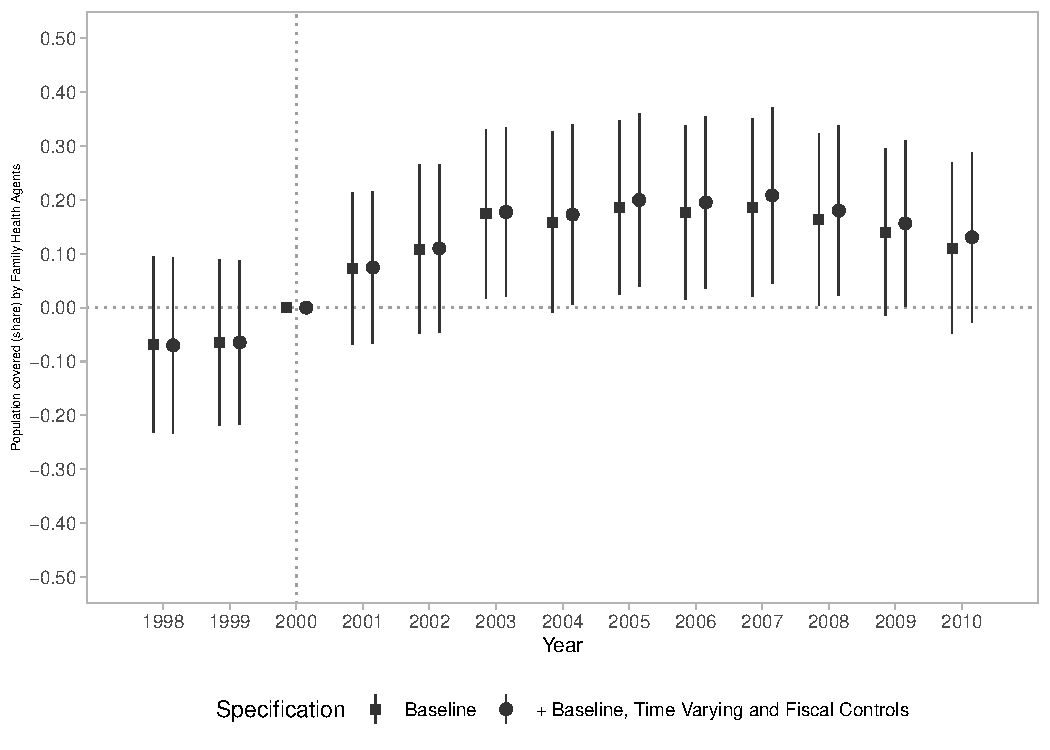
\includegraphics[width=\textwidth]{plots/eSF_popprop_dist_ec29_baseline_dist_ec29_baseline_11.pdf}
    \end{subfigure}
    
    \end{center}
    
\end{figure}

\begin{figure}[h!]
    \begin{center}
    \caption{Effects on Primary Care Coverage - Intensive Margin}\label{fig:12}
    \begin{subfigure}{0.32\textwidth}
        \caption{\scriptsize N. of People Visited}\label{fig:12a}
        \centering
        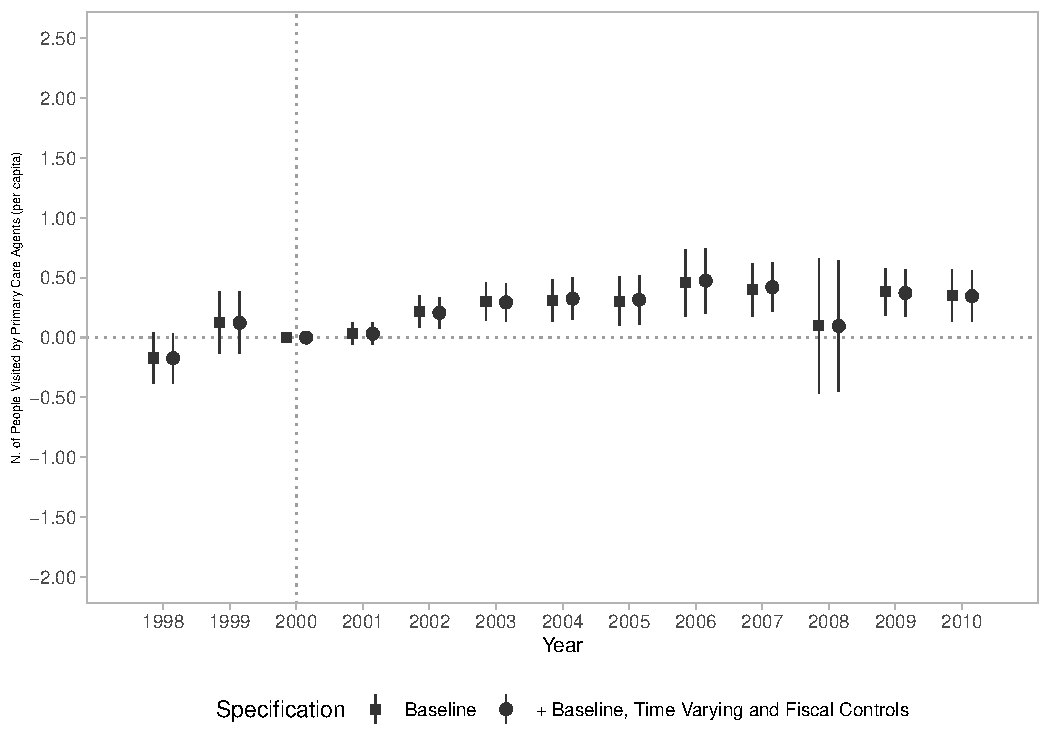
\includegraphics[width=\textwidth]{plots/siab_accomp_especif_pcapita_dist_ec29_baseline_dist_ec29_baseline_12.pdf}
    \end{subfigure}
    \begin{subfigure}{0.32\textwidth}
        \centering
        \caption{\scriptsize People Visited by CH Agents}\label{fig:12b}
        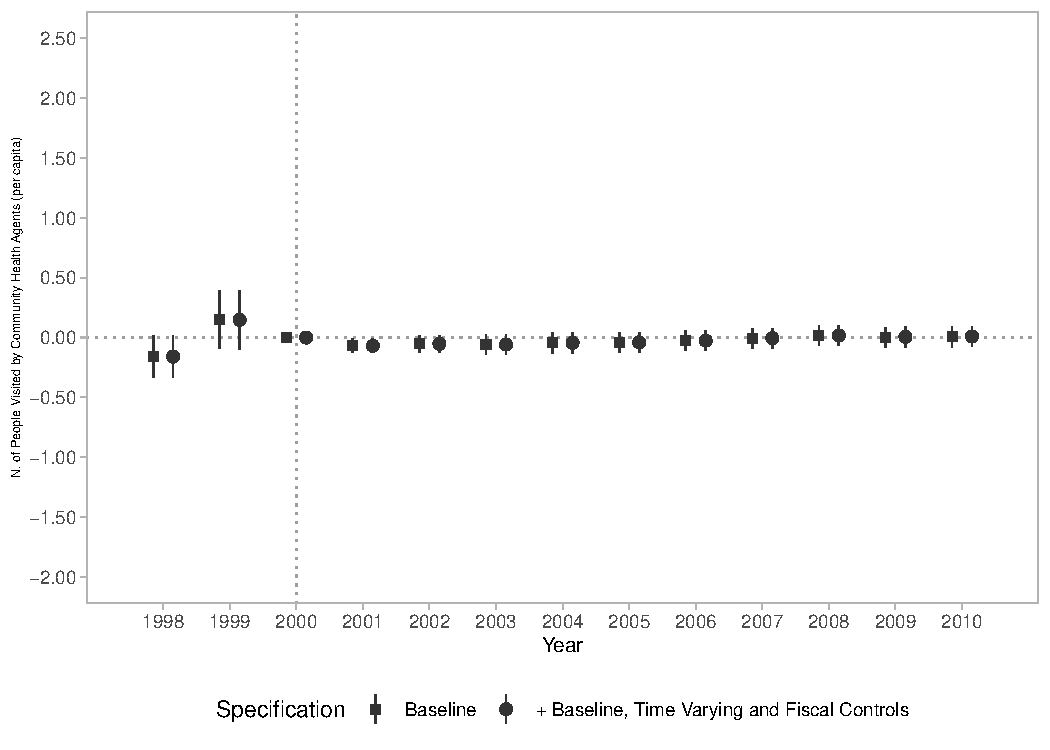
\includegraphics[width=\textwidth]{plots/siab_accomp_especif_pacs_pcapita_dist_ec29_baseline_dist_ec29_baseline_12.pdf}
    \end{subfigure}
    \begin{subfigure}{0.32\textwidth}
        \centering
        \caption{\scriptsize People Visited by FH Agents}\label{fig:12c}
        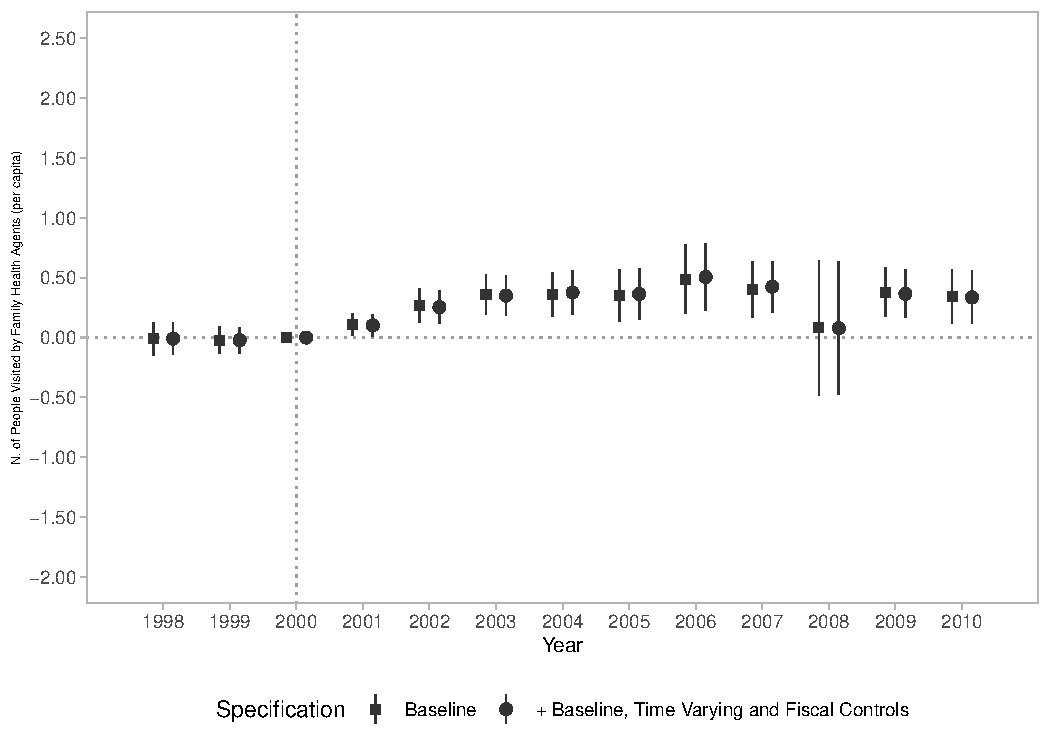
\includegraphics[width=\textwidth]{plots/siab_accomp_especif_psf_pcapita_dist_ec29_baseline_dist_ec29_baseline_12.pdf}
    \end{subfigure}
        \begin{subfigure}{0.32\textwidth}
        \caption{\scriptsize N. of Household Visits}\label{fig:12d}
        \centering
        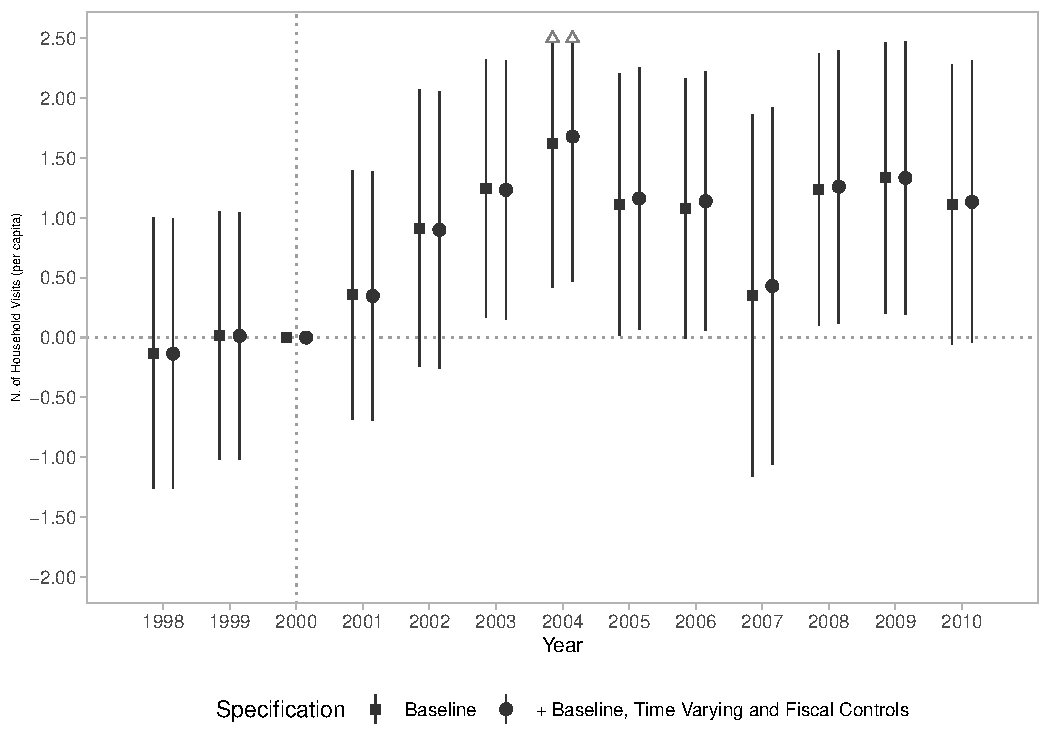
\includegraphics[width=\textwidth]{plots/siab_visit_cha_pcapita_dist_ec29_baseline_dist_ec29_baseline_12.pdf}
    \end{subfigure}
    \begin{subfigure}{0.32\textwidth}
        \centering
        \caption{\scriptsize N. of Household Visits by CH Agents}\label{fig:12e}
        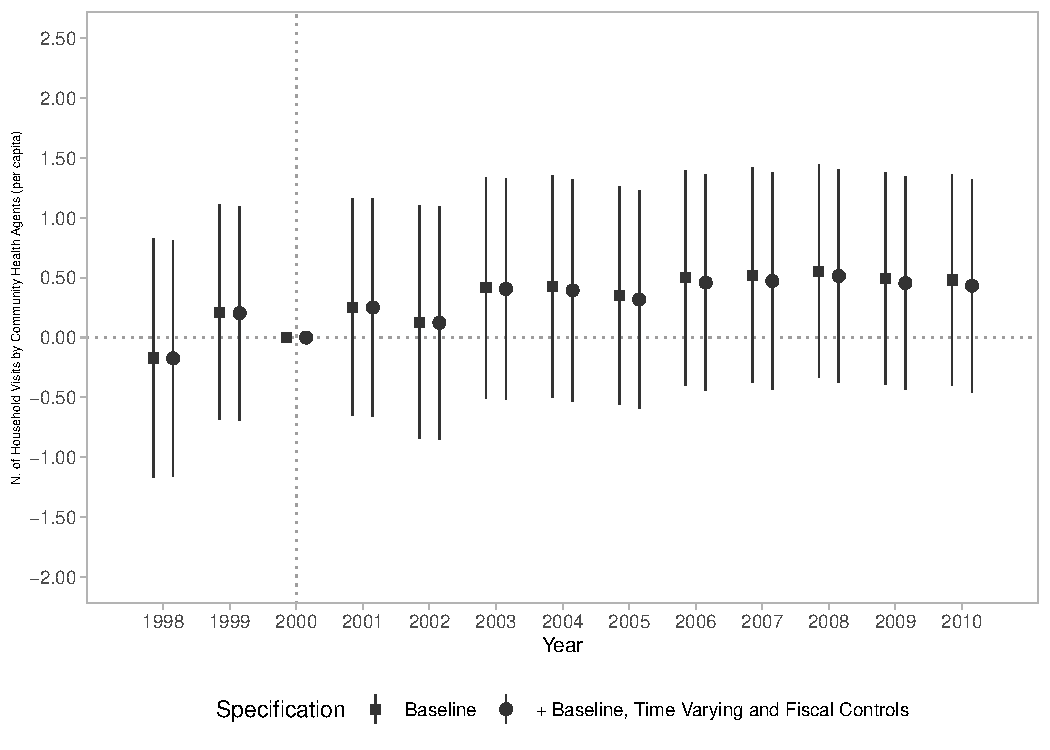
\includegraphics[width=\textwidth]{plots/siab_visit_cha_pacs_pcapita_dist_ec29_baseline_dist_ec29_baseline_12.pdf}
    \end{subfigure}
    \begin{subfigure}{0.32\textwidth}
        \centering
        \caption{\scriptsize N. of Household Visits by FH Agents}\label{fig:12f}
        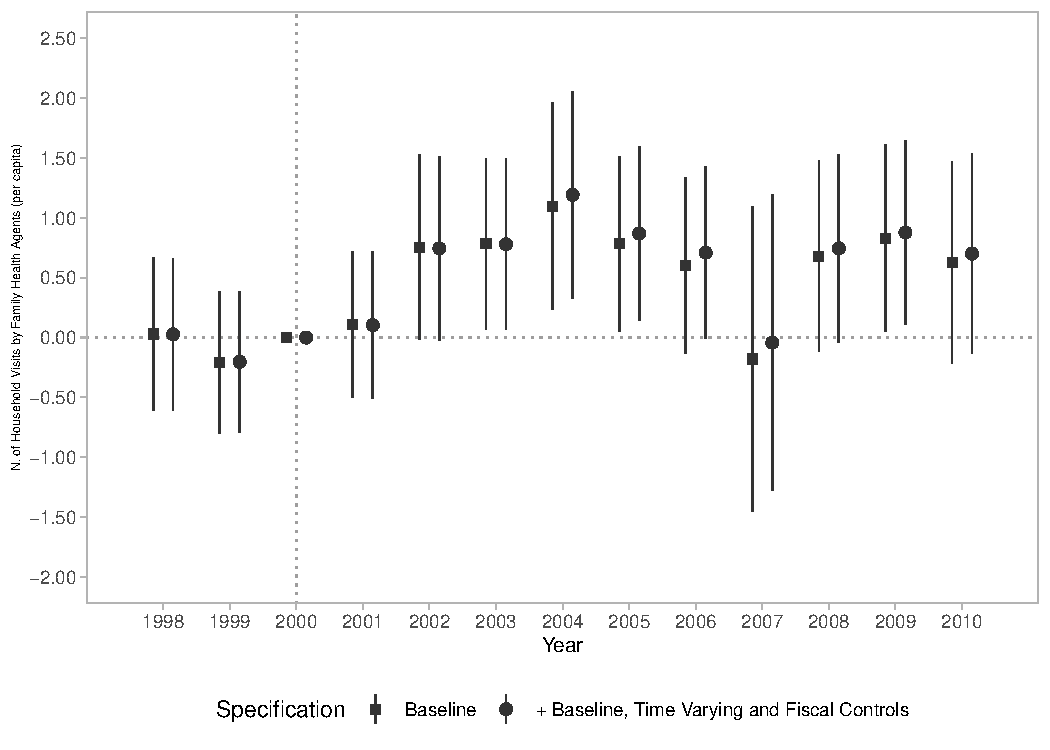
\includegraphics[width=\textwidth]{plots/siab_visit_cha_psf_pcapita_dist_ec29_baseline_dist_ec29_baseline_12.pdf}
    \end{subfigure}
        \begin{subfigure}{0.32\textwidth}
        \caption{\scriptsize N. of Appointments}\label{fig:12g}
        \centering
        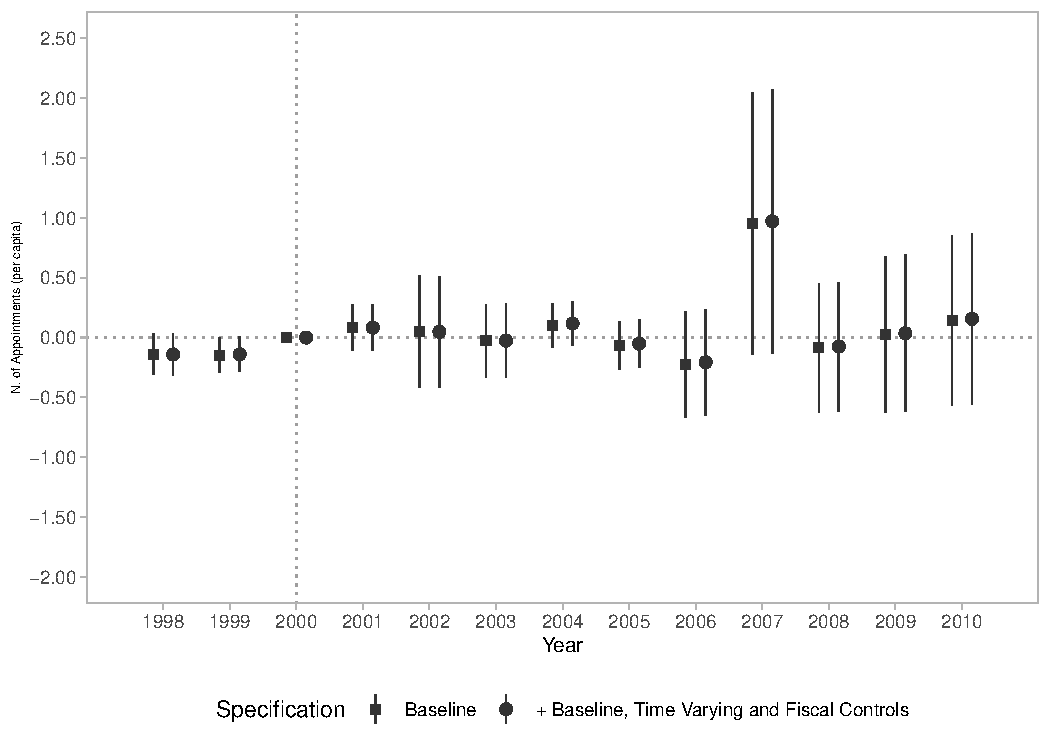
\includegraphics[width=\textwidth]{plots/siab_cons_especif_pcapita_dist_ec29_baseline_dist_ec29_baseline_12.pdf}
    \end{subfigure}
    \begin{subfigure}{0.32\textwidth}
        \centering
        \caption{\scriptsize N. of Appointments from CH Program}\label{fig:12h}
        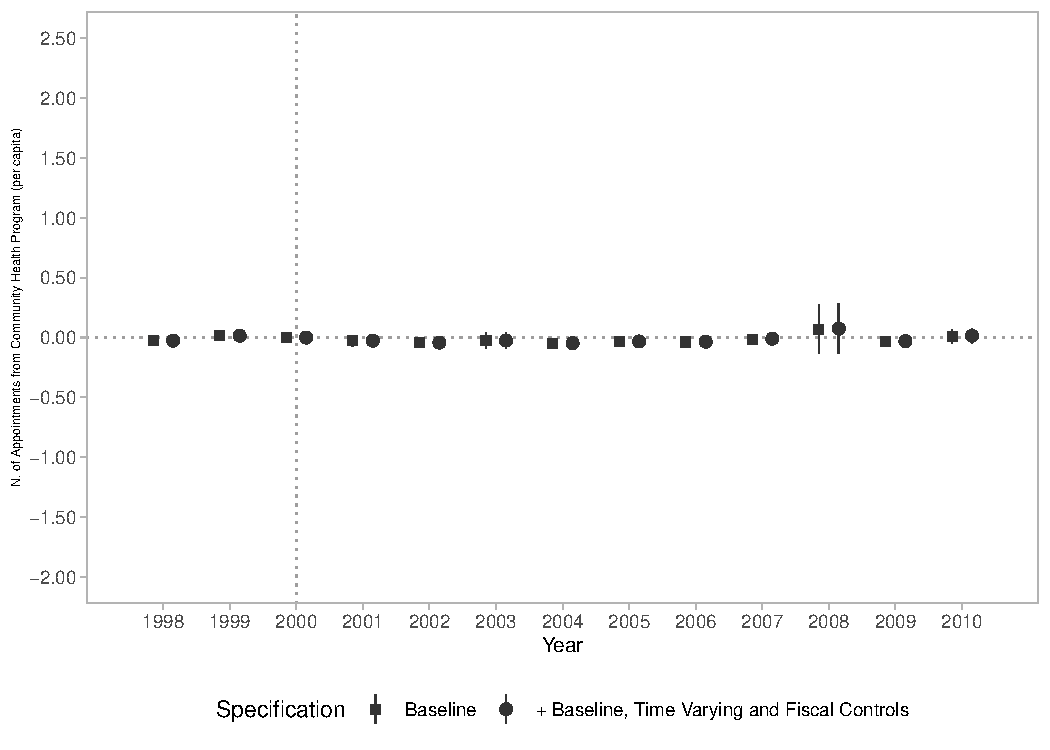
\includegraphics[width=\textwidth]{plots/siab_cons_especif_pacs_pcapita_dist_ec29_baseline_dist_ec29_baseline_12.pdf}
    \end{subfigure}
    \begin{subfigure}{0.32\textwidth}
        \centering
        \caption{\scriptsize N. of Appointments from FH Program}\label{fig:12i}
        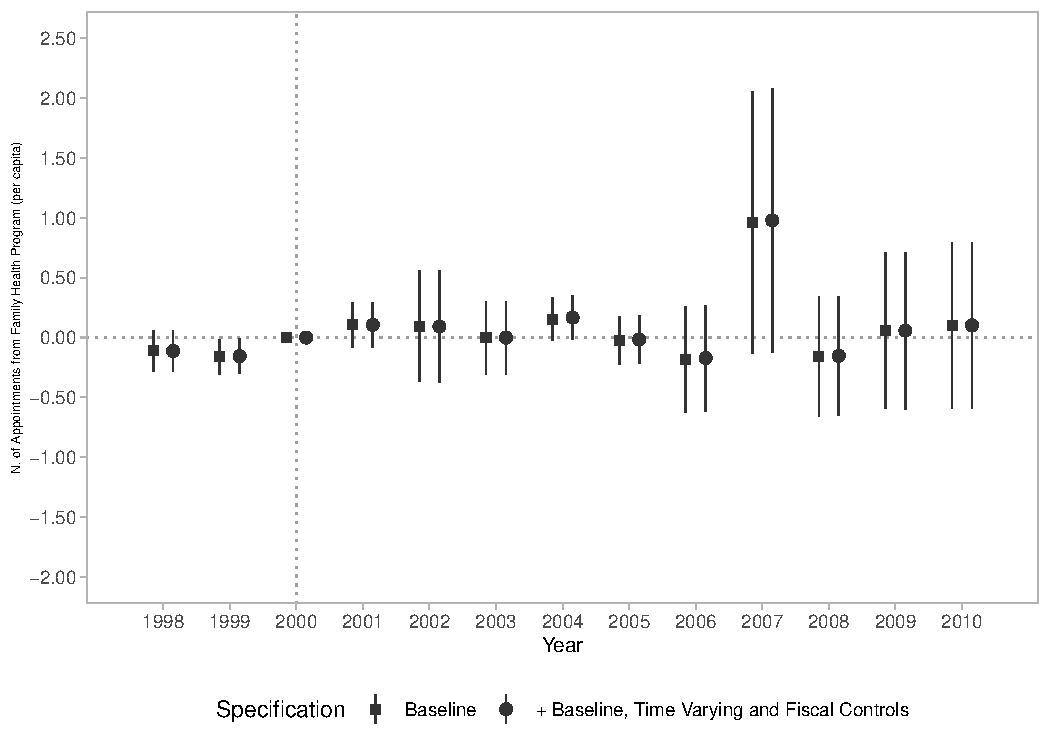
\includegraphics[width=\textwidth]{plots/siab_cons_especif_psf_pcapita_dist_ec29_baseline_dist_ec29_baseline_12.pdf}
    \end{subfigure}
    
    \end{center}
    
\end{figure}

\begin{figure}[h!]
    \begin{center}
    \caption{Effects on Access to Health Services}\label{fig:13}
    \begin{subfigure}{0.48\textwidth}
        \caption{\scriptsize Prenatal Visits Ignored}\label{fig:13a}
        \centering
        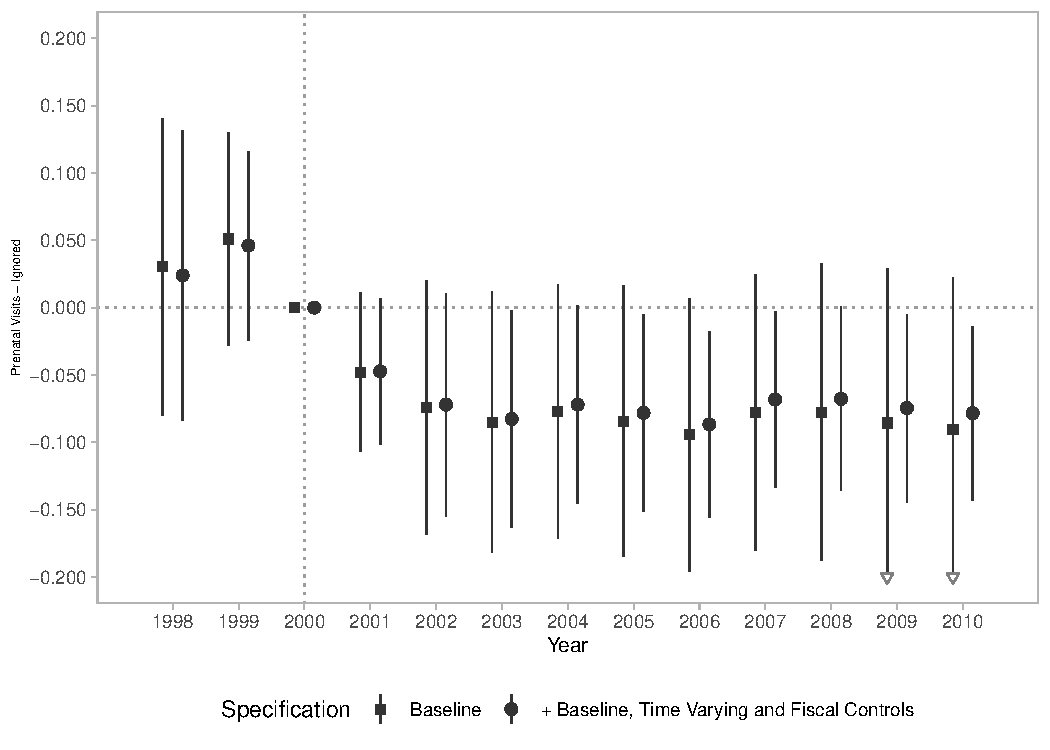
\includegraphics[width=\textwidth]{plots/birth_prenat_ig_dist_ec29_baseline_dist_ec29_baseline_13.pdf}
    \end{subfigure}
    \begin{subfigure}{0.48\textwidth}
        \caption{\scriptsize Prenatal Visits None}\label{fig:13b}
        \centering
        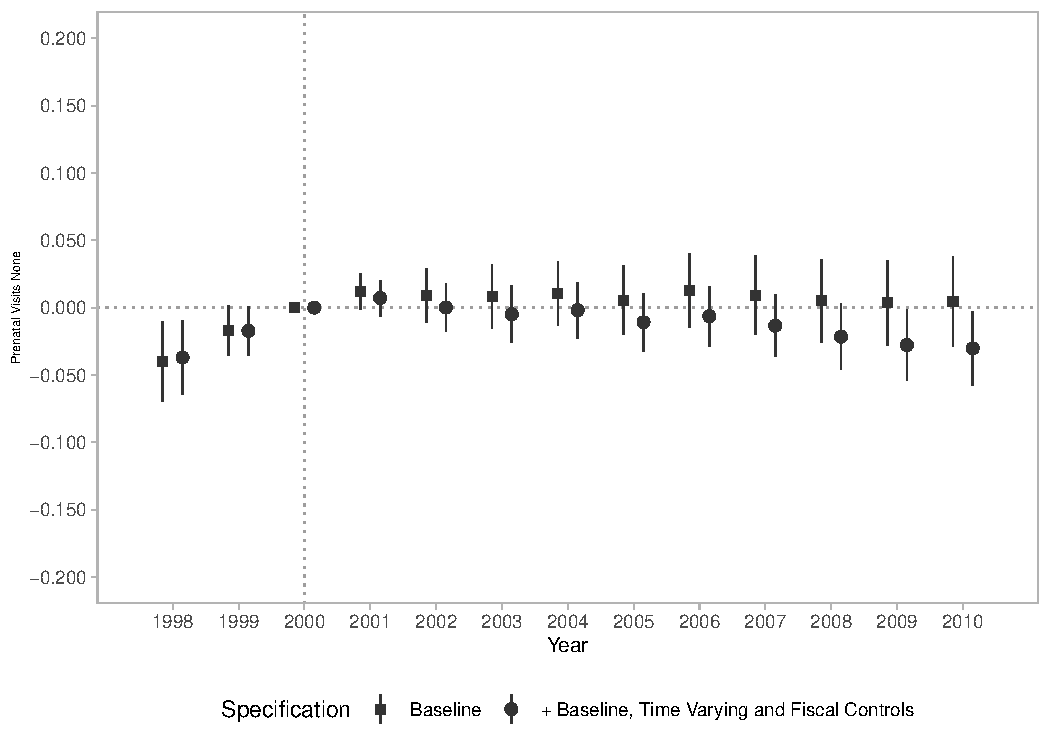
\includegraphics[width=\textwidth]{plots/birth_prenat_0_dist_ec29_baseline_dist_ec29_baseline_13.pdf}
    \end{subfigure}
    \begin{subfigure}{0.48\textwidth}
        \centering
        \caption{\scriptsize Prenatal Visits 1-6}\label{fig:13c}
        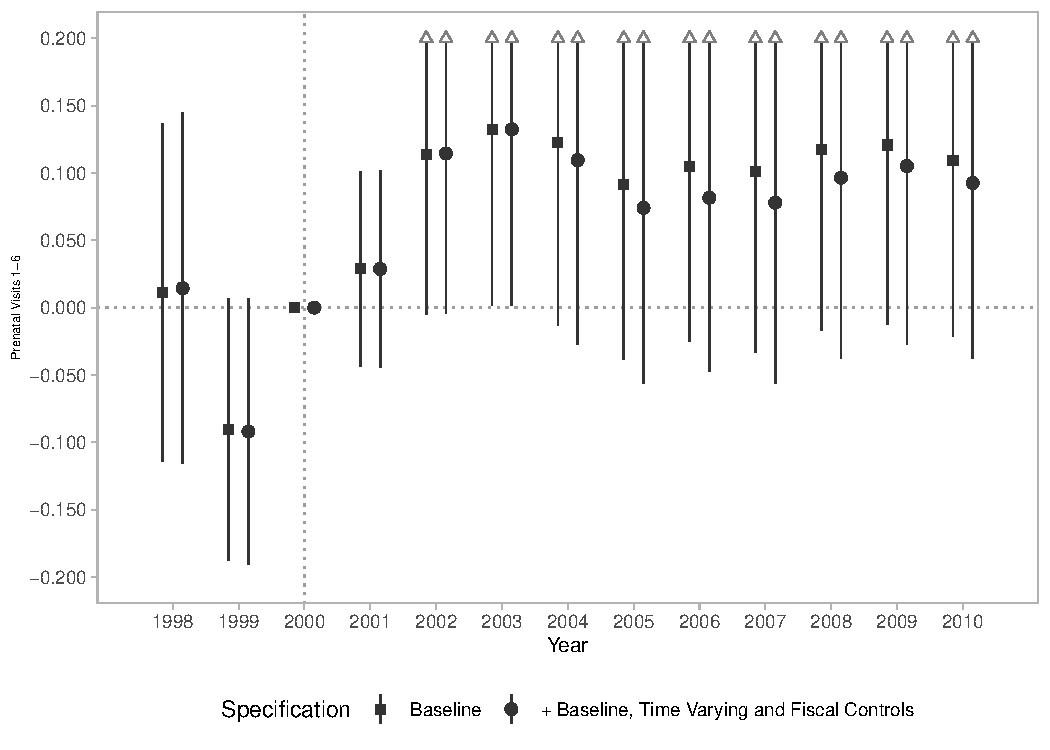
\includegraphics[width=\textwidth]{plots/birth_prenat_1_6_dist_ec29_baseline_dist_ec29_baseline_13.pdf}
    \end{subfigure}
    \begin{subfigure}{0.48\textwidth}
        \centering
        \caption{\scriptsize Prenatal Visits 7+}\label{fig:13d}
        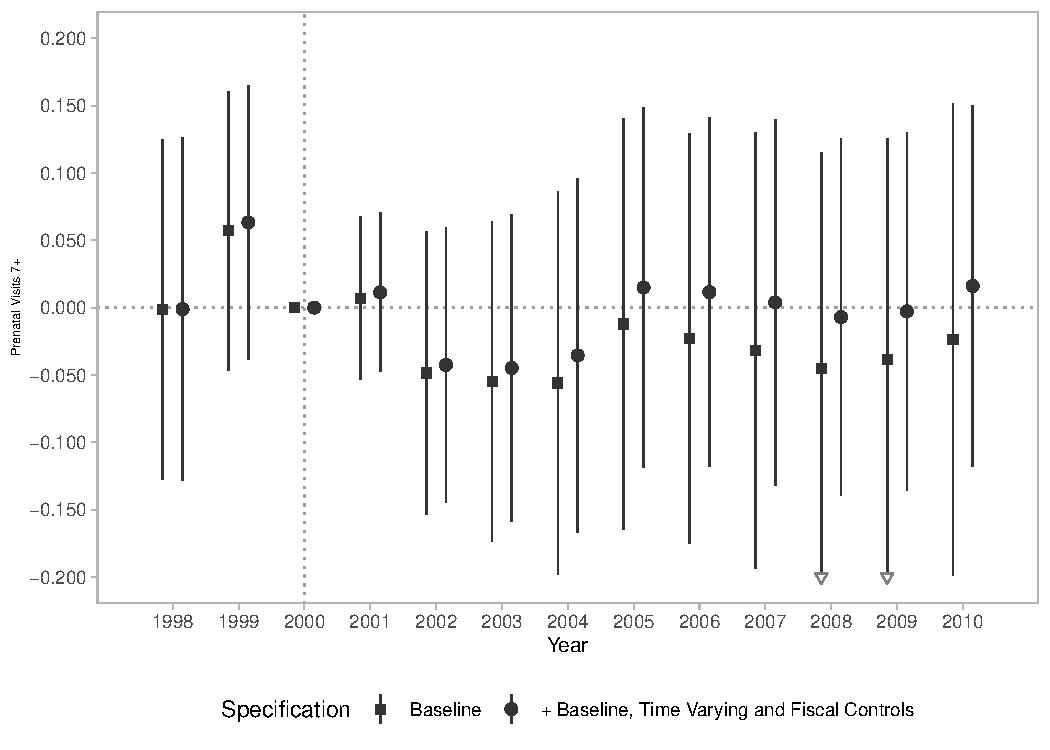
\includegraphics[width=\textwidth]{plots/birth_prenat_7_plus_dist_ec29_baseline_dist_ec29_baseline_13.pdf}
    \end{subfigure}
        
    
    \end{center}
    
    \scriptsize{Notes: The number of observations is 64481. DiD Estimates from Equation \ref{eq:2}. Independent variable is the distance to the EC/29 target in p.p. Square dots represent the baseline model with municipality and state-year fixed effects. Round dots represent fully saturated specification (Column 4 in regression Tables). Lines represent 95\% confidence intervals. Arrows, when present, indicate confidence intervals out of the plot bounds. Standard errors are clustered in the municipality level.}

    
\end{figure}

Table \ref{table:production}, Figures \ref{fig:15} \ref{fig:14}

\begin{table}[H]
\begin{footnotesize}
\begin{center}
\scalebox{0.8}{
\begin{threeparttable}[b]

  \centering
  \caption{Ambulatorial Production and Access to Health Services}
     \begin{tabular}{rrrrrr}
          &       &       &       &       &  \\
    \midrule
    \midrule
          &       & \multicolumn{4}{c}{Distance to EC9 target} \\
\cmidrule{3-6}          &       & \multicolumn{1}{c}{(1)} & \multicolumn{1}{c}{(2)} & \multicolumn{1}{c}{(3)} & \multicolumn{1}{c}{(4)} \\
    \midrule
    \multicolumn{1}{p{26.355em}}{\textbf{A. Ambulatorial Production}} &       &       &       &       &  \\
    \multicolumn{1}{l}{\multirow{2}[0]{*}{Outpatient procedures per capita}} &       & \multicolumn{1}{c}{2.67***} & \multicolumn{1}{c}{2.473**} & \multicolumn{1}{c}{2.544**} & \multicolumn{1}{c}{ 2.528** } \\
          &       & \multicolumn{1}{c}{(1.027)} & \multicolumn{1}{c}{(1.025)} & \multicolumn{1}{c}{(1.021)} & \multicolumn{1}{c}{ (1.019) } \\
    \multicolumn{1}{l}{\multirow{2}[0]{*}{Primary Care Outpatient procedures per capita}} &       & \multicolumn{1}{c}{2.231**} & \multicolumn{1}{c}{2.228**} & \multicolumn{1}{c}{2.282**} & \multicolumn{1}{c}{ 2.266** } \\
          &       & \multicolumn{1}{c}{(0.944)} & \multicolumn{1}{c}{(0.934)} & \multicolumn{1}{c}{(0.931)} & \multicolumn{1}{c}{ (0.929) } \\
    \multicolumn{1}{l}{\multirow{2}[0]{*}{N. of Low \& Mid Complexity Outpatient Procedures (per capita)}} &       & \multicolumn{1}{c}{2.337**} & \multicolumn{1}{c}{2.225**} & \multicolumn{1}{c}{2.331***} & \multicolumn{1}{c}{ 2.337*** } \\
          &       & \multicolumn{1}{c}{(0.908)} & \multicolumn{1}{c}{(0.898)} & \multicolumn{1}{c}{(0.892)} & \multicolumn{1}{c}{ (0.891) } \\
    \multicolumn{1}{l}{\multirow{2}[0]{*}{N. of High Complexity Outpatient Procedures (per capita)}} &       & \multicolumn{1}{c}{-0.136} & \multicolumn{1}{c}{-0.191} & \multicolumn{1}{c}{-0.174} & \multicolumn{1}{c}{ -0.177 } \\
          &       & \multicolumn{1}{c}{(0.134)} & \multicolumn{1}{c}{(0.133)} & \multicolumn{1}{c}{(0.132)} & \multicolumn{1}{c}{ (0.132) } \\
    \multicolumn{1}{l}{\multirow{2}[0]{*}{N. of Outpatient Procedures by Low Skilled Workers (per capita)}} &       & \multicolumn{1}{c}{0.04} & \multicolumn{1}{c}{0.019} & \multicolumn{1}{c}{0.074} & \multicolumn{1}{c}{ 0.074 } \\
          &       & \multicolumn{1}{c}{(0.354)} & \multicolumn{1}{c}{(0.346)} & \multicolumn{1}{c}{(0.343)} & \multicolumn{1}{c}{ (0.342) } \\
    \multicolumn{1}{l}{\multirow{2}[0]{*}{N. of Outpatient procedures by Mid Skilled Workers (per capita)}} &       & \multicolumn{1}{c}{0.383} & \multicolumn{1}{c}{0.346} & \multicolumn{1}{c}{0.353} & \multicolumn{1}{c}{ 0.351 } \\
          &       & \multicolumn{1}{c}{(0.481)} & \multicolumn{1}{c}{(0.479)} & \multicolumn{1}{c}{(0.479)} & \multicolumn{1}{c}{ (0.479) } \\
          &       &       &       &       &  \\
    \midrule
    \multicolumn{1}{p{26.355em}}{\textbf{B. Access to Health Services}} &       &       &       &       &  \\
    \multicolumn{1}{l}{\multirow{2}[0]{*}{Prenatal Visits None}} &       & \multicolumn{1}{c}{0.025*} & \multicolumn{1}{c}{0.006} & \multicolumn{1}{c}{0.005} & \multicolumn{1}{c}{0.005} \\
          &       & \multicolumn{1}{c}{(0.015)} & \multicolumn{1}{c}{(0.011)} & \multicolumn{1}{c}{(0.011)} & \multicolumn{1}{c}{(0.011)} \\
    \multicolumn{1}{l}{\multirow{2}[0]{*}{Prenatal Visits 1-6}} &       & \multicolumn{1}{c}{0.13**} & \multicolumn{1}{c}{0.121**} & \multicolumn{1}{c}{0.118*} & \multicolumn{1}{c}{0.116*} \\
          &       & \multicolumn{1}{c}{(0.059)} & \multicolumn{1}{c}{(0.061)} & \multicolumn{1}{c}{(0.061)} & \multicolumn{1}{c}{(0.06)} \\
    \multicolumn{1}{l}{\multirow{2}[0]{*}{Prenatal Visits 7+}} &       & \multicolumn{1}{c}{-0.051} & \multicolumn{1}{c}{-0.034} & \multicolumn{1}{c}{-0.03} & \multicolumn{1}{c}{-0.029} \\
          &       & \multicolumn{1}{c}{(0.074)} & \multicolumn{1}{c}{(0.062)} & \multicolumn{1}{c}{(0.061)} & \multicolumn{1}{c}{(0.061)} \\
          &       &       &       &       &  \\
    \bottomrule
    \bottomrule
    \end{tabular}%
    
    
  \label{table:production}%

\end{threeparttable}
}
\end{center}
\end{footnotesize}
\end{table}

\begin{figure}[h!]
    \begin{center}
    \caption{Effects on Infant Mortality Rates}\label{fig:15}
    \begin{subfigure}{0.32\textwidth}
        \caption{\scriptsize Total}\label{fig:15a}
        \centering
        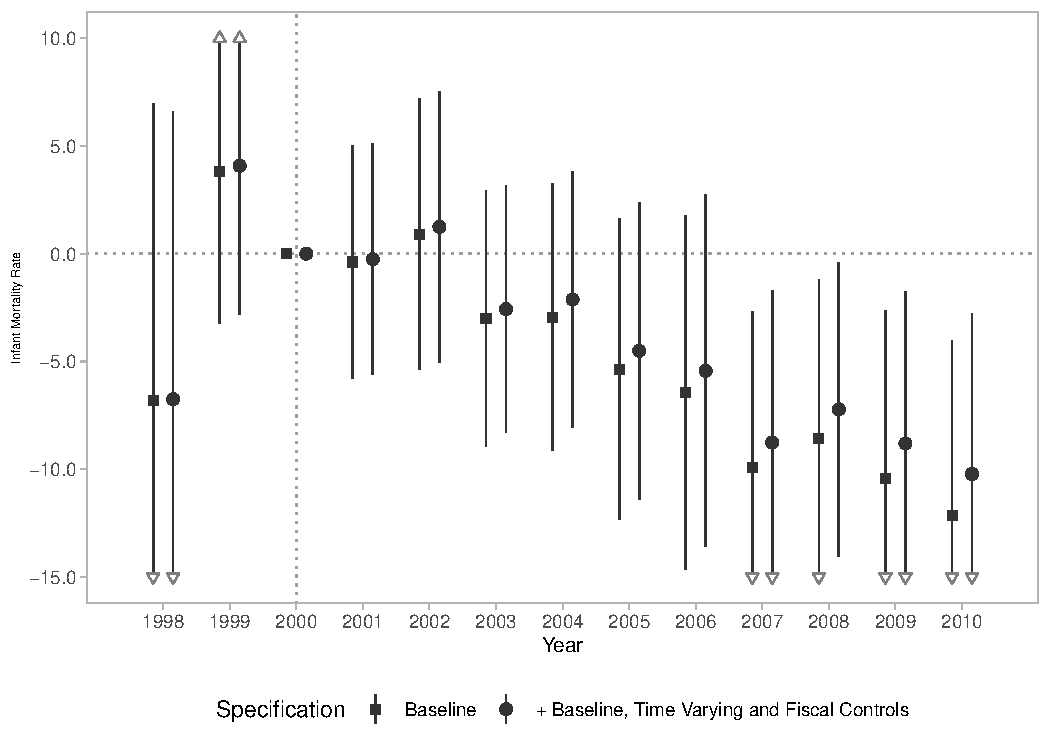
\includegraphics[width=\textwidth]{plots/tx_mi_dist_ec29_baseline_dist_ec29_baseline_15.pdf}
    \end{subfigure}
    \begin{subfigure}{0.32\textwidth}
        \centering
        \caption{\scriptsize Amenable to Primary Care}\label{fig:15b}
        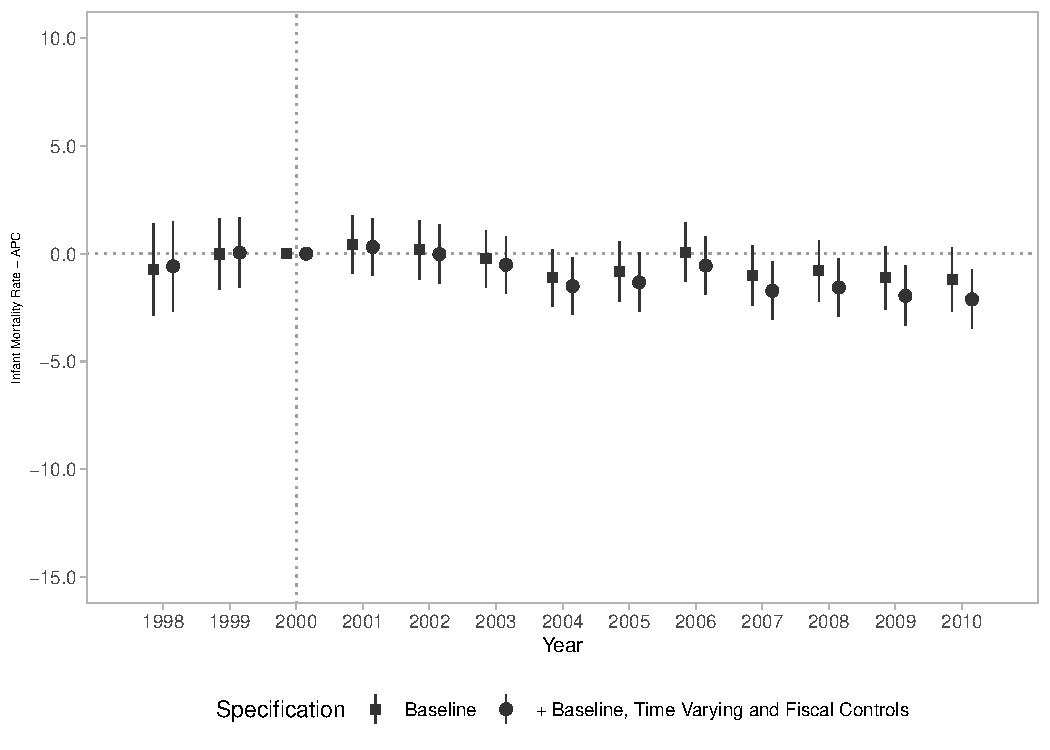
\includegraphics[width=\textwidth]{plots/tx_mi_icsap_dist_ec29_baseline_dist_ec29_baseline_15.pdf}
    \end{subfigure}
    \begin{subfigure}{0.32\textwidth}
        \centering
        \caption{\scriptsize Non-Amenable to Primary Care}\label{fig:15c}
        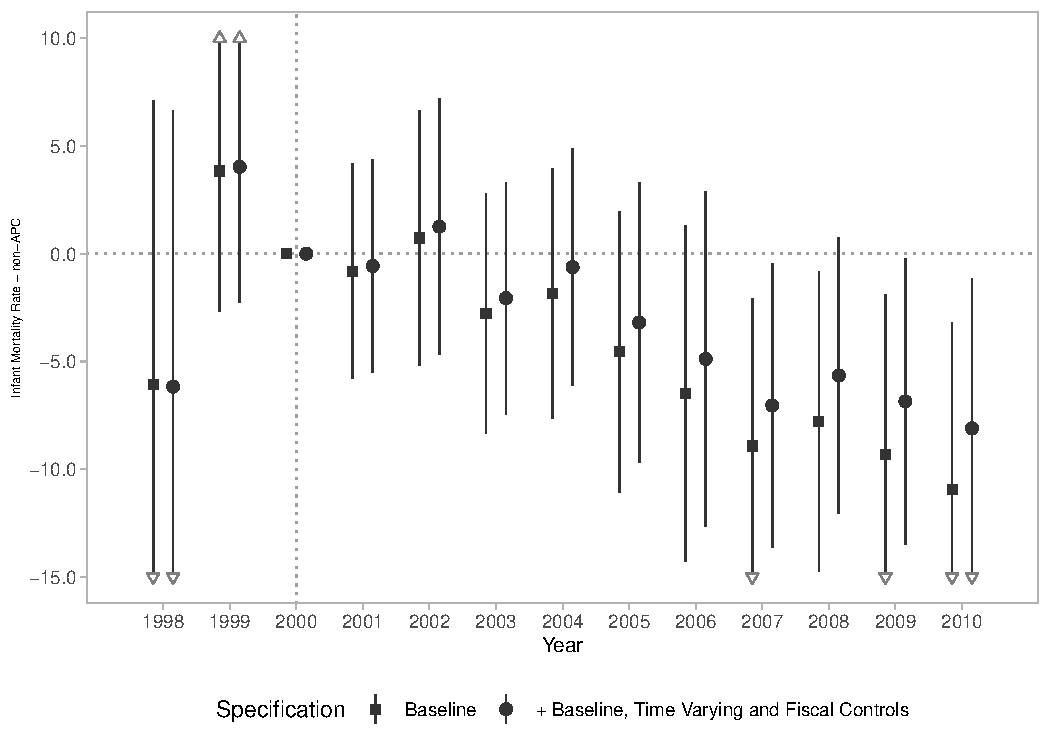
\includegraphics[width=\textwidth]{plots/tx_mi_nicsap_dist_ec29_baseline_dist_ec29_baseline_15.pdf}
    \end{subfigure}
    
    \end{center}
    
        \scriptsize{Notes: The number of observations is 64482. DiD Estimates from Equation \ref{eq:2}. Independent variable is the distance to the EC/29 target in p.p. Square dots represent the baseline model with municipality and state-year fixed effects. Round dots represent fully saturated specification (Column 4 in regression Tables). Lines represent 95\% confidence intervals. Arrows, when present, indicate confidence intervals out of the plot bounds. Standard errors are clustered in the municipality level.}
    
\end{figure}

\begin{figure}[h!]
    \begin{center}
    \caption{Effects on Access to Health Services}\label{fig:14}
    \begin{subfigure}{0.32\textwidth}
        \caption{\scriptsize Prenatal Visits None}\label{fig:14a}
        \centering
        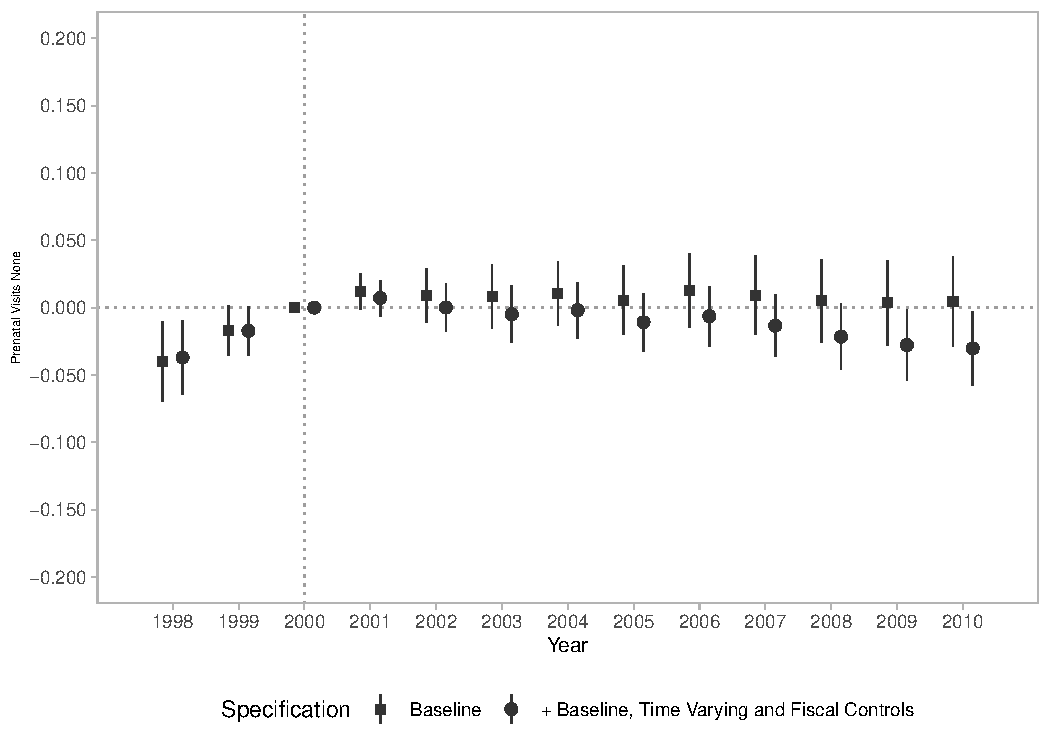
\includegraphics[width=\textwidth]{plots/birth_prenat_0_dist_ec29_baseline_dist_ec29_baseline_14.pdf}
    \end{subfigure}
    \begin{subfigure}{0.32\textwidth}
        \centering
        \caption{\scriptsize Prenatal Visits 1-6}\label{fig:14b}
        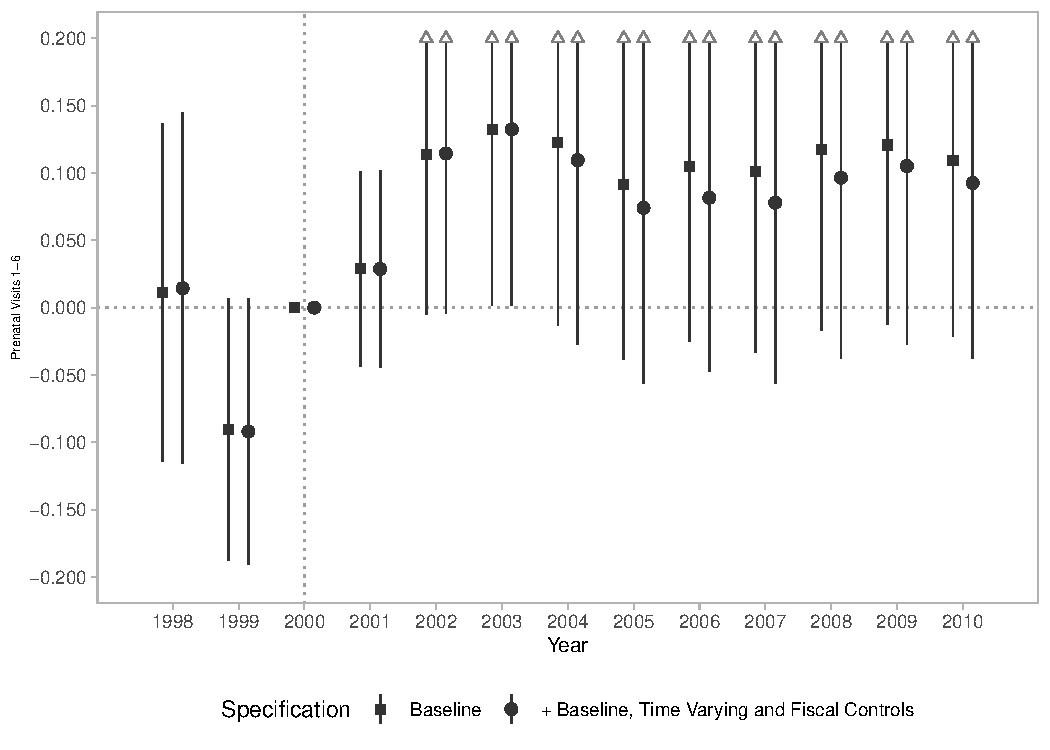
\includegraphics[width=\textwidth]{plots/birth_prenat_1_6_dist_ec29_baseline_dist_ec29_baseline_14.pdf}
    \end{subfigure}
    \begin{subfigure}{0.32\textwidth}
        \centering
        \caption{\scriptsize Prenatal Visits 7+}\label{fig:14c}
        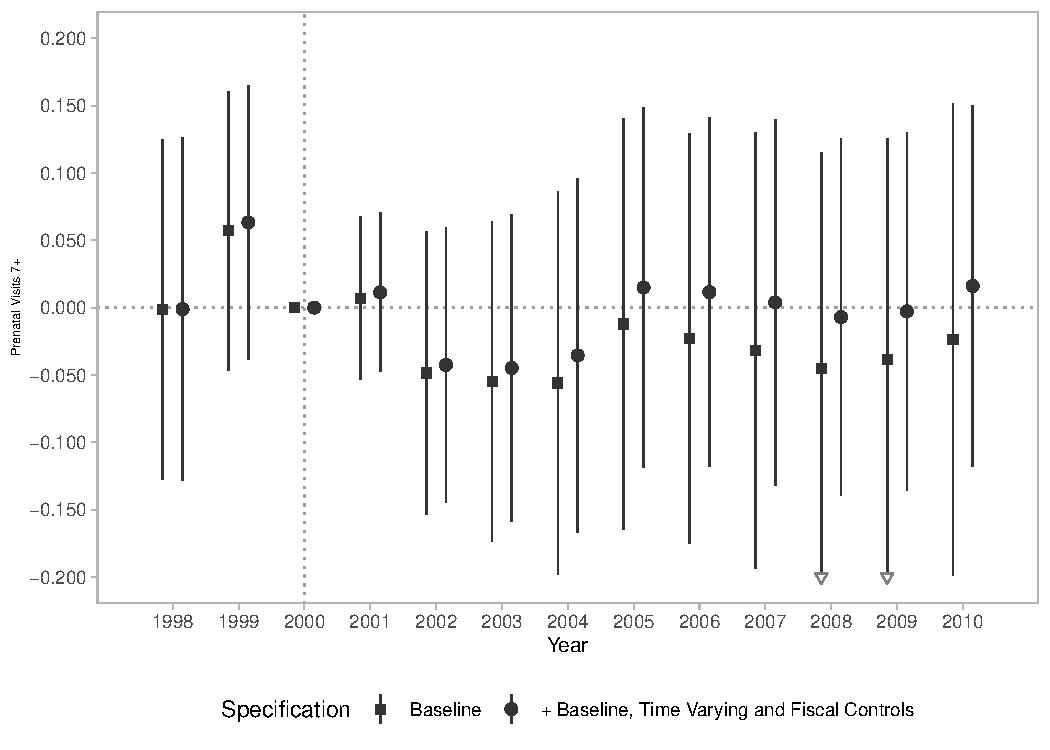
\includegraphics[width=\textwidth]{plots/birth_prenat_7_plus_dist_ec29_baseline_dist_ec29_baseline_14.pdf}
    \end{subfigure}
        
    
    \end{center}
    
\end{figure}

\subsection{Effects on Infant Mortality}

Having provided evidence of meaningful increases in health spending, we now present estimates of the causal effects on infant mortality. Differently from most of the literature linking health spending with infant mortality \citep{filmer1999,bokhari2007,moreno2015,nixon2006,gupta2002effectiveness,cremieux1999,bokhari2007}, we are able to assess the effects not only for total infant mortality rates, but also for rates by timing of death, rates by cause of death, and also infant mortality rates that are amenable to primary care. These results are presented in Table \ref{table:imr}. In our preferred specification, with the exception of ill-defined infant mortality, all outcomes present negative point estimates, but only infant mortality rate within 24 hours and infant mortality rate by infectious diseases present marginally significant estimates. Relative to the baseline mortality rates, a 10\% distance to the target is associated with a reduction of around 3.5\% for mortality within 24 hours and a reduction of around 5\% for mortality due to infectious diseases. 

Though most of the continuous DiD estimates for Infant Mortality Rates presented in Table \ref{table:imr} are not statistically significant, the more flexible coefficients estimated with equation \ref{eq:2} provide useful information on the dynamics of the effects and suggest the presence of some significant reduction in infant mortality rates. The estimates of these regressions and its confidence intervals of 5\% are presented in Figures \ref{fig:imr1}, \ref{fig:imr2} and \ref{fig:imr3}. Total infant mortality rate (\ref{fig:imr1_a}) and infant mortality rate amenable to primary care (\ref{fig:imr1_b}) present a clear trend of reduction, with estimates for later years being statistically significant. Mortality from 1 to 27 days old (Figure \ref{fig:imr2_c} and from 27 days to one year old (Figure \ref{fig:imr2_d} presents some evidence of reduction through the years after treatment. When it comes to infant mortality rates by cause of death, mortality due to perinatal conditions (Figure \ref{fig:imr3_c}) presents a clear trend of reduction with all years from 2005 on presenting statistically significant estimates.

In general, articles estimating the causal relationship between health spending and mortality run log-log regressions and present estimates for the elasticity of mortality with respect to health spending. We explicitly choose not to apply transformations to our health outcomes variables due to the amount of observations with values equal to 0, notably the ones related to birth and mortality. As we work with a data set comprising all the Brazilian municipalities with available data for the period of analyses, some with population size as little as 700 inhabitants, it is common to find infant mortality rates of 0. Running log transformation would throw away some relevant information for several outcomes. Nonetheless, to relate our results to the literature on this topic we estimate "back of the envelope" elasticities for all mortality rates presented so far. Table \ref{table:elasticity} presents these elasticities for our preferred specification estimates using Finbra Health and Sanitation Spending per capita and Infant Mortality Rates. 

Figures \ref{fig:16} \ref{fig:17} \ref{fig:18}

\begin{table}[h!]
\begin{footnotesize}
\begin{center}
\scalebox{0.9}{
\begin{threeparttable}[b]

  \centering
  \caption{Infant Mortality Rates}
     \begin{tabular}{rrcccc}
          &       &       &       &       &  \\
          &       &       &       &       &  \\
    \midrule
    \midrule
          &       & (1)   & (2)   & (3)   & (4) \\
    \midrule
    \multicolumn{1}{p{15.145em}}{\textbf{A. Infant Mortality Rate}} &       &       &       &       &  \\
    \multicolumn{1}{p{15.145em}}{Total} &       & -5.015 & -3.772 & -3.831 & -3.889 \\
          &       & (3.435) & (2.853) & (2.836) & (2.828) \\
    \multicolumn{1}{p{15.145em}}{Amenable to Primary Care} &       & -0.361 & -0.866 & -0.893 & -0.905 \\
          &       & (0.603) & (0.553) & (0.553) & (0.554) \\
    \multicolumn{1}{p{15.145em}}{Non-Amenable to Primary Care} &       & -4.653 & -2.907 & -2.939 & -2.984 \\
          &       & (3.245) & (2.645) & (2.632) & (2.624) \\
          &       &       &       &       &  \\
    \midrule
    \multicolumn{1}{p{15.145em}}{\textbf{B. By timing}} &       &       &       &       &  \\
    \multicolumn{1}{p{15.145em}}{Fetal} &       & -0.008 & -0.007 & -0.008 & -0.008 \\
          &       & (0.008) & (0.008) & (0.008) & (0.008) \\
    \multicolumn{1}{p{15.145em}}{Within 24h} &       & -2.275* & -2.083** & -2.07** & -2.071** \\
          &       & (1.225) & (0.98) & (0.979) & (0.976) \\
    \multicolumn{1}{p{15.145em}}{1 to 27 days} &       & -4.228* & -2.883 & -2.911 & -2.922 \\
          &       & (2.555) & (2.064) & (2.052) & (2.046) \\
    \multicolumn{1}{p{15.145em}}{27 days to 1 year} &       & -0.787 & -0.89 & -0.92 & -0.967 \\
          &       & (1.435) & (1.248) & (1.246) & (1.243) \\
          &       &       &       &       &  \\
    \midrule
    \multicolumn{1}{p{15.145em}}{\textbf{C. By Cause of Death}} &       &       &       &       &  \\
    \multicolumn{1}{p{15.145em}}{Infectious} &       & -0.374 & -0.811 & -0.82 & -0.831 \\
          &       & (0.567) & (0.535) & (0.535) & (0.534) \\
    \multicolumn{1}{p{15.145em}}{Respiratory} &       & -0.494 & -0.507 & -0.511 & -0.517 \\
          &       & (0.474) & (0.411) & (0.409) & (0.409) \\
    \multicolumn{1}{p{15.145em}}{Perinatal} &       & -5.349** & -3.648* & -3.69* & -3.707* \\
          &       & (2.571) & (2.015) & (2.007) & (2.002) \\
    \multicolumn{1}{p{15.145em}}{Congenital} &       & -0.235 & -0.169 & -0.16 & -0.157 \\
          &       & (0.463) & (0.436) & (0.434) & (0.434) \\
    \multicolumn{1}{p{15.145em}}{External} &       & 0.024 & -0.049 & -0.037 & -0.034 \\
          &       & (0.183) & (0.165) & (0.165) & (0.166) \\
    \multicolumn{1}{p{15.145em}}{Nutritional} &       & -0.204 & -0.328 & -0.33 & -0.343 \\
          &       & (0.246) & (0.231) & (0.232) & (0.232) \\
    \multicolumn{1}{p{15.145em}}{Other} &       & -0.183 & -0.123 & -0.132 & -0.139 \\
          &       & (0.201) & (0.199) & (0.198) & (0.198) \\
    \multicolumn{1}{p{15.145em}}{Ill-Defined} &       & 1.8** & 1.862** & 1.849** & 1.84** \\
          &       & (0.849) & (0.776) & (0.779) & (0.779) \\
          &       &       &       &       &  \\
    \bottomrule
    \bottomrule
    \end{tabular}%
    
    
    \begin{tablenotes}
  \scriptsize{\underline{Notes}: The number of observations is 64482. DiD Estimates from Equation \ref{eq:1}. Independent variable is the distance to the EC/29 target in p.p. Column 1 presents the baseline model with municipality and state-year fixed effects. Column 2 adds baseline socioeconomic controls from the Census interacted with time. Column 3 adds controls for GDP per capita and \emph{Bolsa Familia} transfers per capita. Column 4 adds fiscal controls. Covariates omitted. Standard errors in brackets are clustered in the municipality level. ∗p < 0.10, ∗ ∗ p < 0.05, ∗ ∗ ∗p < 0.01}
  \end{tablenotes}
    
    
  \label{table:imr}%

\end{threeparttable}
}
\end{center}
\end{footnotesize}
\end{table}

\begin{figure}[h!]
    \begin{center}
    \caption{Effects on Infant Mortality Rates - By Timing}\label{fig:16}
    \begin{subfigure}{0.48\textwidth}
        \caption{\scriptsize Fetal}\label{fig:16a}
        \centering
        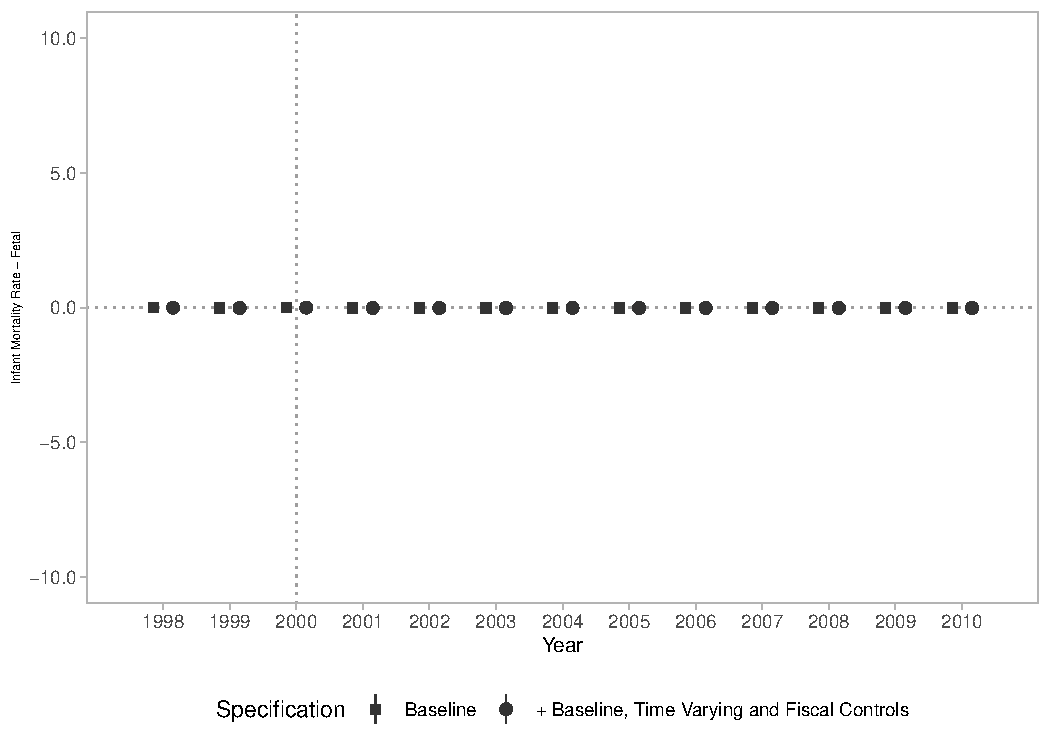
\includegraphics[width=\textwidth]{plots/tx_mi_fet_dist_ec29_baseline_dist_ec29_baseline_16.pdf}
    \end{subfigure}
    \begin{subfigure}{0.48\textwidth}
        \centering
        \caption{\scriptsize Within 24h}\label{fig:16b}
        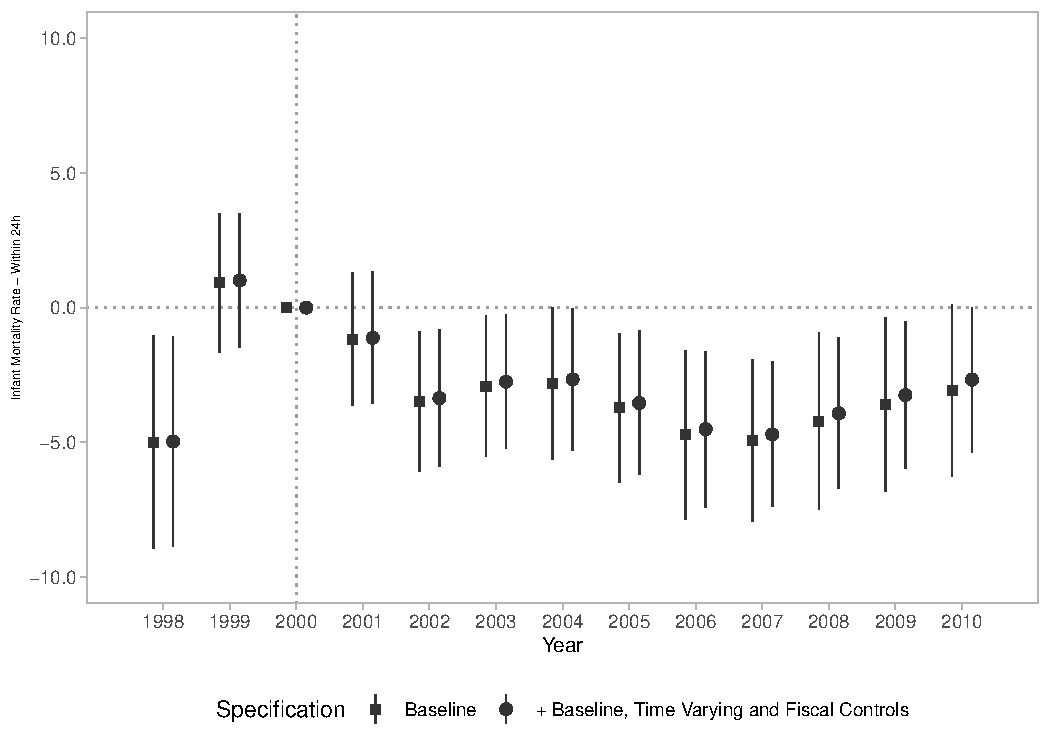
\includegraphics[width=\textwidth]{plots/tx_mi_24h_dist_ec29_baseline_dist_ec29_baseline_16.pdf}
    \end{subfigure}
    \begin{subfigure}{0.48\textwidth}
        \centering
        \caption{\scriptsize 1 to 27 days}\label{fig:16c}
        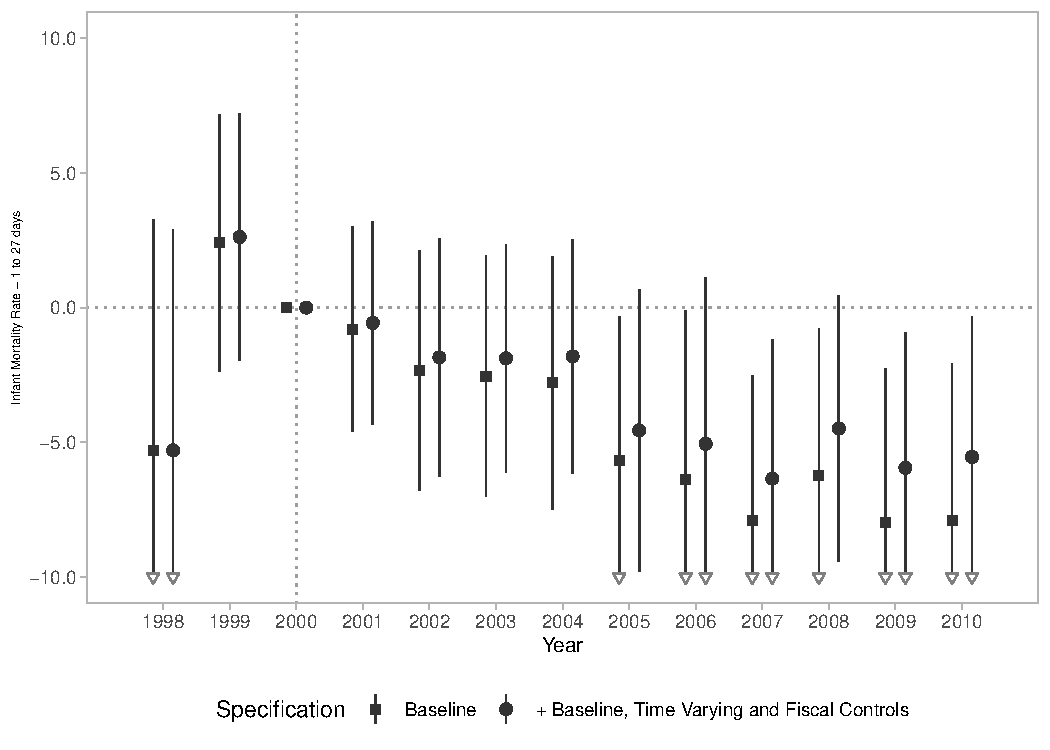
\includegraphics[width=\textwidth]{plots/tx_mi_27d_dist_ec29_baseline_dist_ec29_baseline_16.pdf}
    \end{subfigure}
    \begin{subfigure}{0.48\textwidth}
        \centering
        \caption{\scriptsize 27 days to 1 year}\label{fig:16d}
        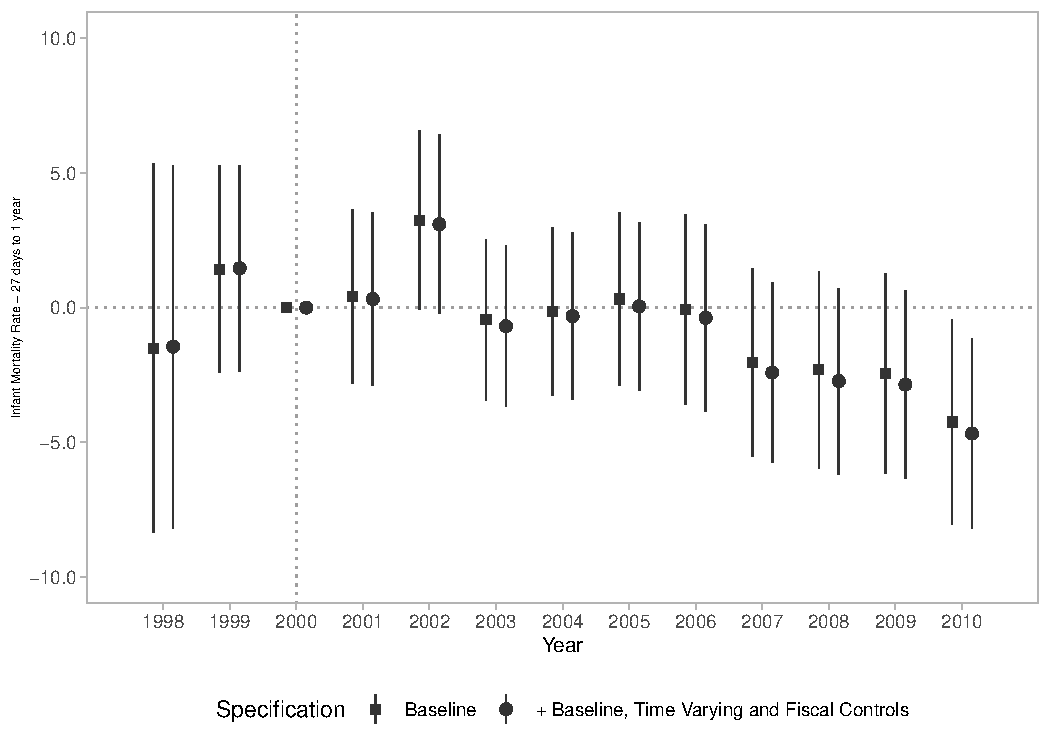
\includegraphics[width=\textwidth]{plots/tx_mi_ano_dist_ec29_baseline_dist_ec29_baseline_16.pdf}
    \end{subfigure}
    
    \end{center}
    
            \scriptsize{Notes: The number of observations is 64482. DiD Estimates from Equation \ref{eq:2}. Independent variable is the distance to the EC/29 target in p.p. Square dots represent the baseline model with municipality and state-year fixed effects. Round dots represent fully saturated specification (Column 4 in regression Tables). Lines represent 95\% confidence intervals. Arrows, when present, indicate confidence intervals out of the plot bounds. Standard errors are clustered in the municipality level.}
    
\end{figure}

\begin{figure}[h!]
    \begin{center}
    \caption{Effects on Infant Mortality Rates - By Timing}\label{fig:17}
    \begin{subfigure}{0.48\textwidth}
        \caption{\scriptsize Fetal}\label{fig:17a}
        \centering
        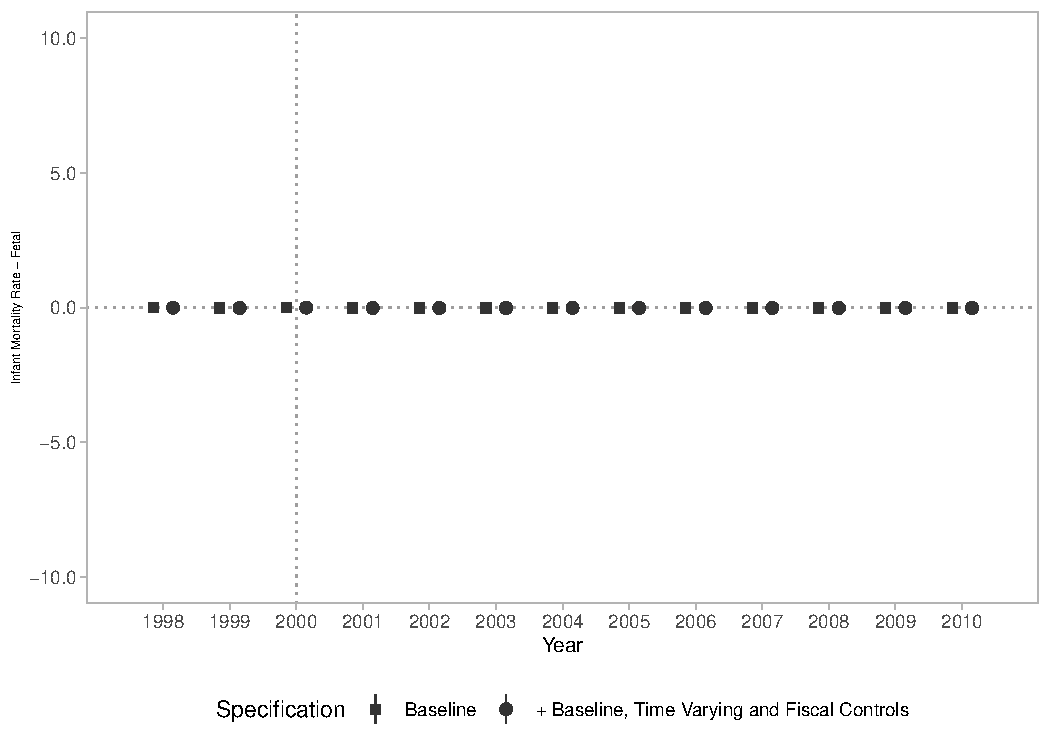
\includegraphics[width=\textwidth]{plots/tx_mi_fet_dist_ec29_baseline_dist_ec29_baseline_17.pdf}
    \end{subfigure}
    \begin{subfigure}{0.48\textwidth}
        \centering
        \caption{\scriptsize Within 24h}\label{fig:17b}
        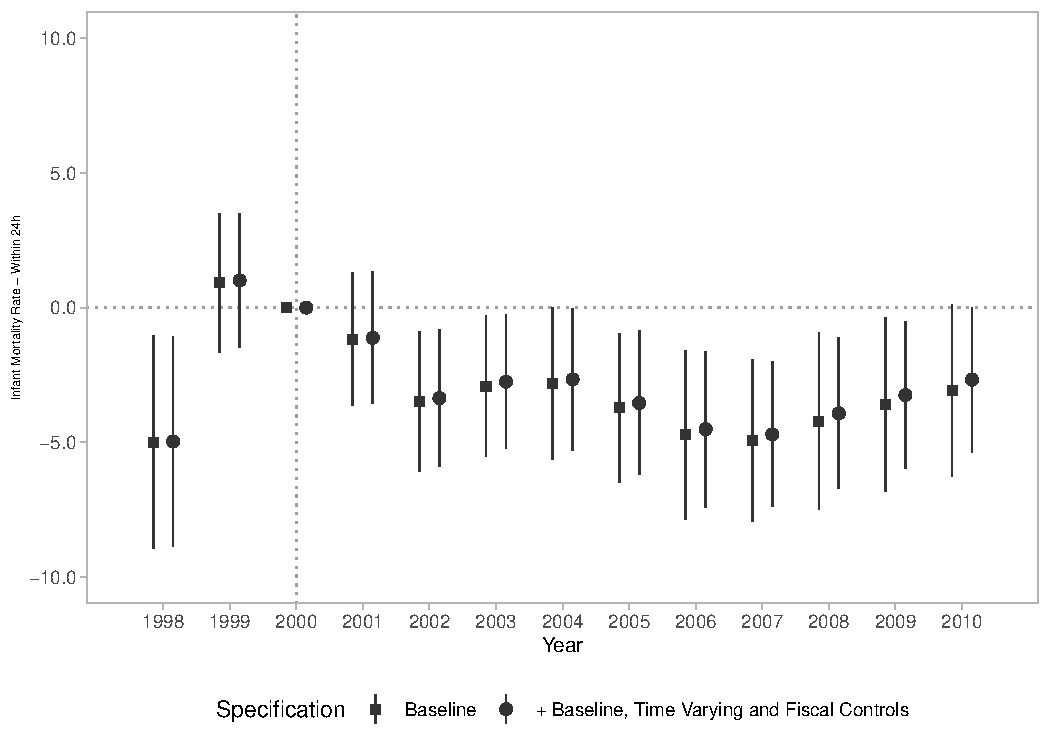
\includegraphics[width=\textwidth]{plots/tx_mi_24h_dist_ec29_baseline_dist_ec29_baseline_17.pdf}
    \end{subfigure}
    \begin{subfigure}{0.48\textwidth}
        \centering
        \caption{\scriptsize 1 to 27 days}\label{fig:17c}
        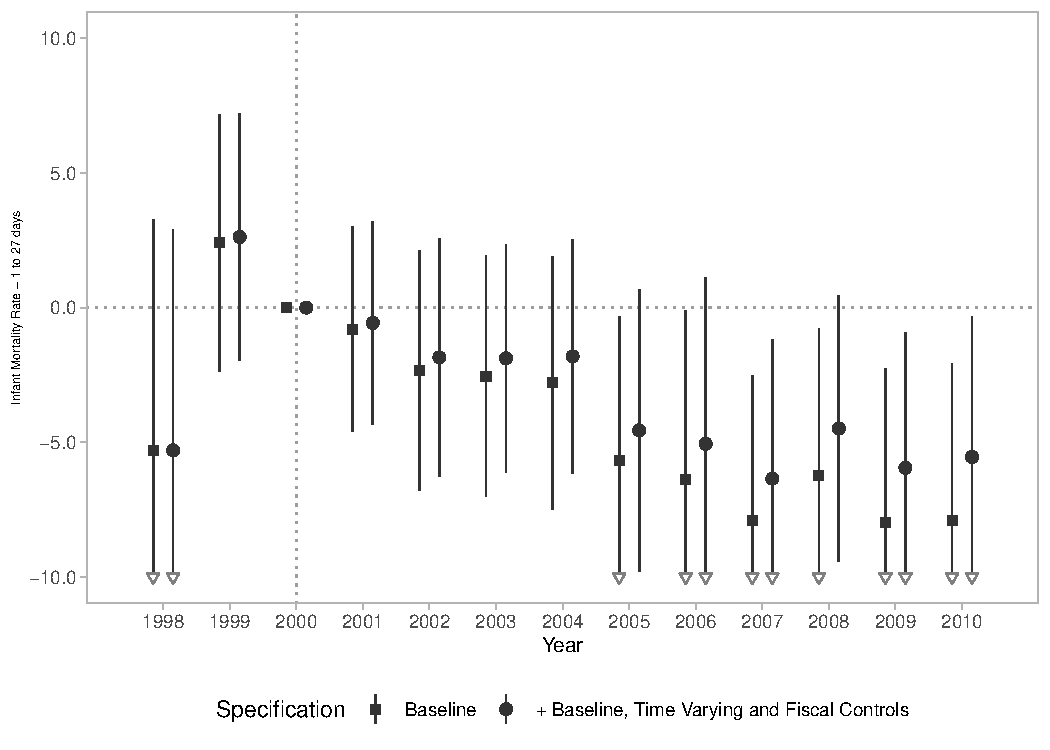
\includegraphics[width=\textwidth]{plots/tx_mi_27d_dist_ec29_baseline_dist_ec29_baseline_17.pdf}
    \end{subfigure}
    \begin{subfigure}{0.48\textwidth}
        \centering
        \caption{\scriptsize 27 days to 1 year}\label{fig:17d}
        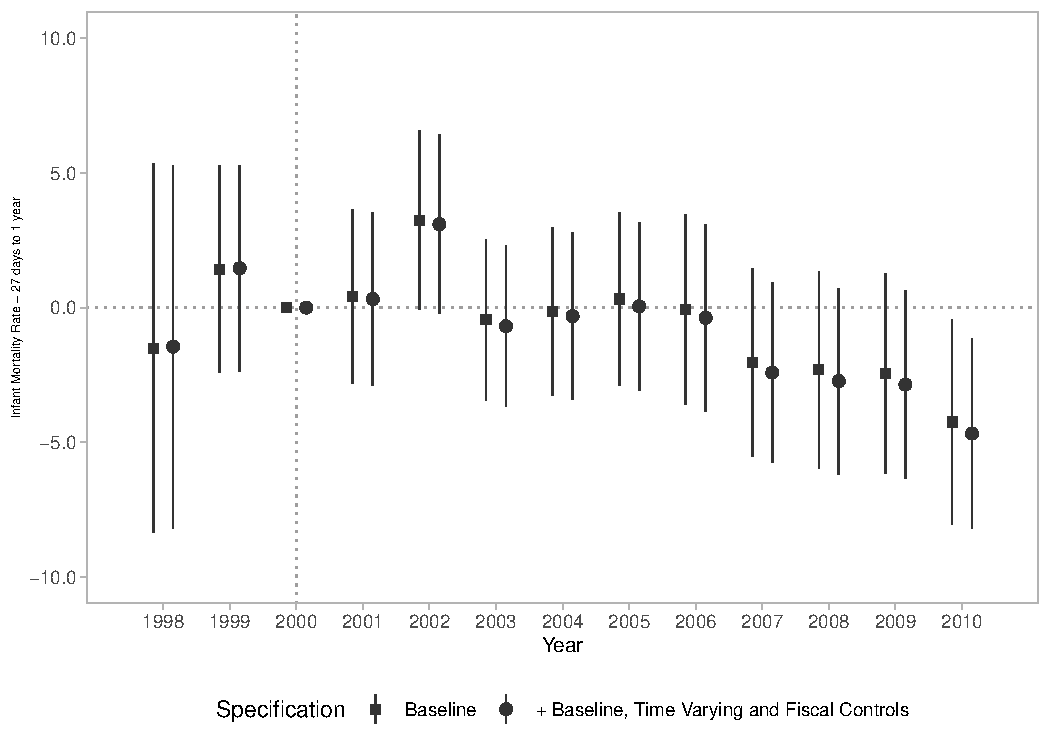
\includegraphics[width=\textwidth]{plots/tx_mi_ano_dist_ec29_baseline_dist_ec29_baseline_17.pdf}
    \end{subfigure}
    
    \end{center}
    
\end{figure}

\begin{figure}[h!]
    \begin{center}
    \caption{Effects on Infant Mortality Rates - By Cause}\label{fig:18}
    \begin{subfigure}{0.32\textwidth}
        \caption{\scriptsize Infectious}\label{fig:18a}
        \centering
        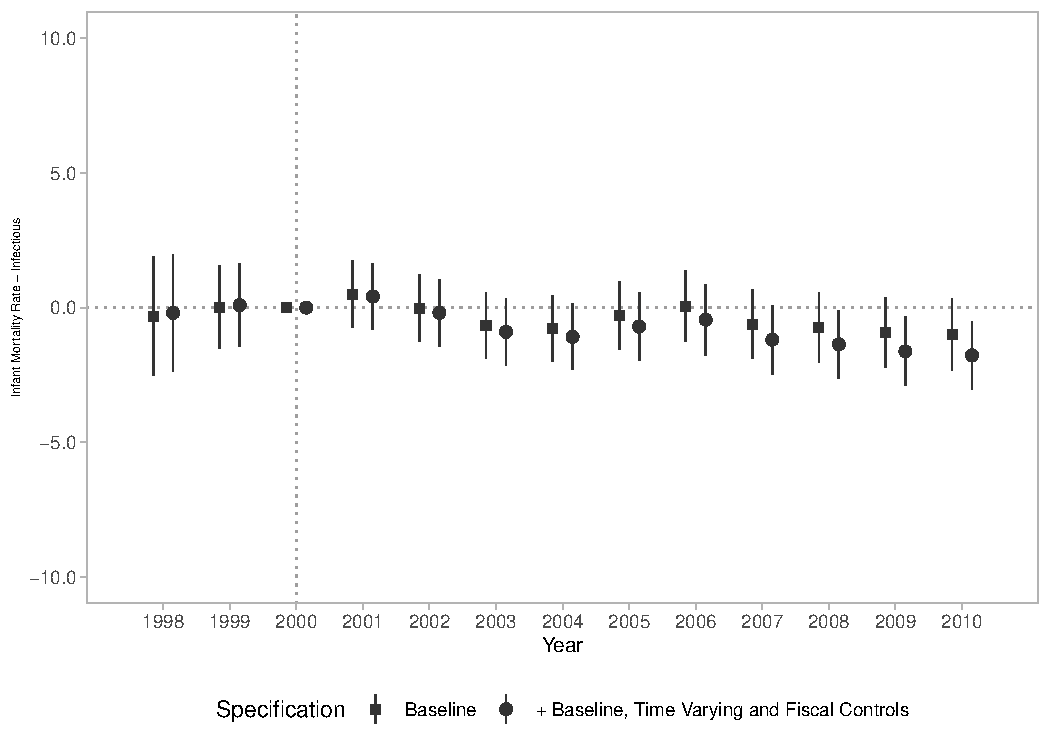
\includegraphics[width=\textwidth]{plots/tx_mi_infec_dist_ec29_baseline_dist_ec29_baseline_18.pdf}
    \end{subfigure}
    \begin{subfigure}{0.32\textwidth}
        \centering
        \caption{\scriptsize Respiratory}\label{fig:18b}
        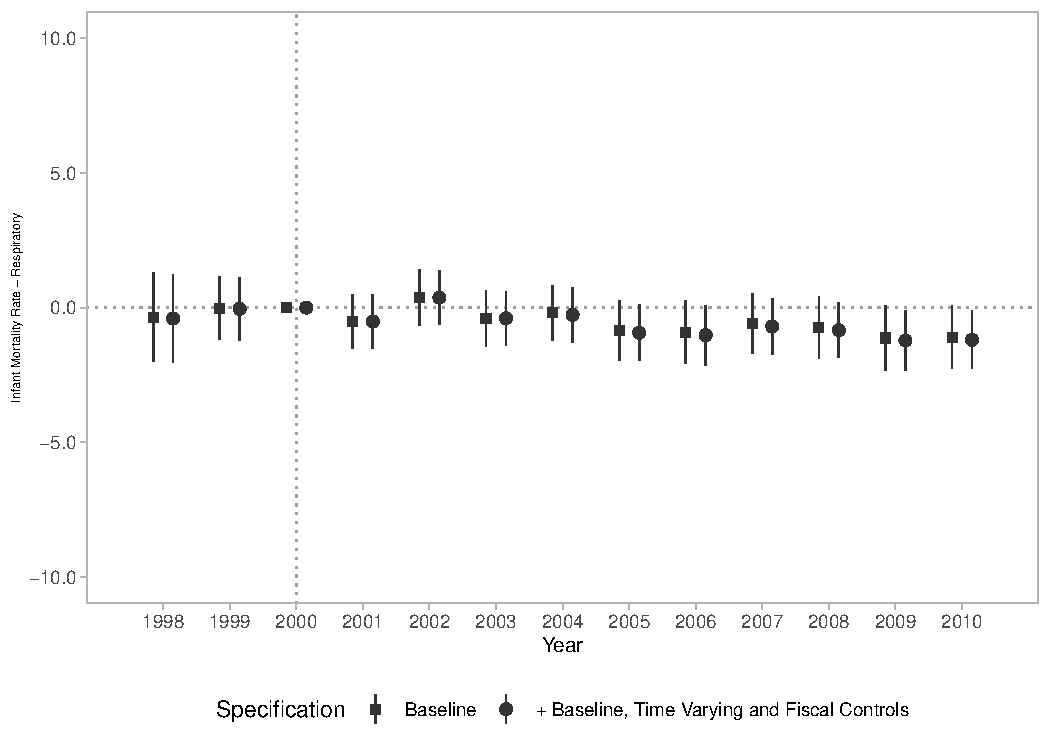
\includegraphics[width=\textwidth]{plots/tx_mi_resp_dist_ec29_baseline_dist_ec29_baseline_18.pdf}
    \end{subfigure}
    \begin{subfigure}{0.32\textwidth}
        \centering
        \caption{\scriptsize Perinatal}\label{fig:18c}
        \includegraphics[width=\textwidth]{plots/tx_mi_perinat_dist_ec29_baseline_dist_ec29_baseline_18.pdf}
    \end{subfigure}
        \begin{subfigure}{0.32\textwidth}
        \centering
        \caption{\scriptsize Congenital}\label{fig:18d}
        \includegraphics[width=\textwidth]{plots/tx_mi_cong_dist_ec29_baseline_dist_ec29_baseline_18.pdf}
    \end{subfigure}
        \begin{subfigure}{0.32\textwidth}
        \centering
        \caption{\scriptsize External}\label{fig:18e}
        \includegraphics[width=\textwidth]{plots/tx_mi_ext_dist_ec29_baseline_dist_ec29_baseline_18.pdf}
    \end{subfigure}
        \begin{subfigure}{0.32\textwidth}
        \centering
        \caption{\scriptsize Nutritional}\label{fig:18f}
        \includegraphics[width=\textwidth]{plots/tx_mi_nut_dist_ec29_baseline_dist_ec29_baseline_18.pdf}
    \end{subfigure}
        \begin{subfigure}{0.32\textwidth}
        \centering
        \caption{\scriptsize Other}\label{fig:18g}
        \includegraphics[width=\textwidth]{plots/tx_mi_out_dist_ec29_baseline_dist_ec29_baseline_18.pdf}
    \end{subfigure}
        \begin{subfigure}{0.32\textwidth}
        \centering
        \caption{\scriptsize Ill-defined}\label{fig:18h}
        \includegraphics[width=\textwidth]{plots/tx_mi_illdef_dist_ec29_baseline_dist_ec29_baseline_18.pdf}
    \end{subfigure}
    \end{center}
    
\end{figure}


[Compare with other articles elasticities]


Table \ref{table:birth} presents the estimates for a few Birth Outcomes. In general, the point estimates are in the expected direction, substantially small, and statistically insignificant.      

Figure \ref{fig:19}

\begin{table}[h!]
\begin{footnotesize}
\begin{center}
\scalebox{0.8}{
\begin{threeparttable}[b]

  \centering
  \caption{Fertility and Birth Outcomes}
     \begin{tabular}{rrcccr}
          &       &       &       &       &  \\
          &       &       &       &       &  \\
    \midrule
    \midrule
          &       & (1)   & (2)   & (3)   & \multicolumn{1}{c}{(4)} \\
    \midrule
    \multicolumn{1}{l}{\textbf{A. Fertility}} &       &       &       &       &  \\
    \multicolumn{1}{p{26.355em}}{Rates of Birth per Woman (10-49y)} &       & 0.009** & 0.008** & 0.009** & \multicolumn{1}{c}{ 0.009** } \\
          &       & (0.004) & (0.003) & (0.003) & \multicolumn{1}{c}{ (0.003) } \\
    \multicolumn{1}{p{26.355em}}{\textbf{B. Birth Outcomes}} &       &       &       &       &  \\
    \multicolumn{1}{p{26.355em}}{Apgar 1} &       & -0.056 & 0.063 & 0.053 & \multicolumn{1}{c}{ 0.051 } \\
          &       & (0.206) & (0.198) & (0.198) & \multicolumn{1}{c}{ (0.198) } \\
    \multicolumn{1}{p{26.355em}}{Apgar 5} &       & 0.009 & 0.107 & 0.104 & \multicolumn{1}{c}{ 0.101 } \\
          &       & (0.183) & (0.179) & (0.18) & \multicolumn{1}{c}{ (0.179) } \\
    \multicolumn{1}{p{26.355em}}{Low Birth Weight (<2.5k)} &       & -0.003 & -0.002 & -0.001 & \multicolumn{1}{c}{ -0.002 } \\
          &       & (0.003) & (0.003) & (0.003) & \multicolumn{1}{c}{ (0.003) } \\
    \multicolumn{1}{p{26.355em}}{Premature Birth} &       & -0.005 & -0.016 & -0.017 & \multicolumn{1}{c}{ -0.017 } \\
          &       & (0.026) & (0.023) & (0.023) & \multicolumn{1}{c}{ (0.023) } \\
    \multicolumn{1}{p{26.355em}}{Sex Ratio at Birth} &       & 0.014 & 0.016 & 0.017 & \multicolumn{1}{c}{ 0.017 } \\
          &       & (0.016) & (0.016) & (0.016) & \multicolumn{1}{c}{ (0.016) } \\
          &       &       &       &       &  \\
    \bottomrule
    \bottomrule
    \end{tabular}%
    
    
    \begin{tablenotes}
  \scriptsize{\underline{Notes}: The number of observations is 64482 for Panel A, 63705 for Apgar 1, 59524 for Apgar 5, 64481 for Low Birth Weight and Premature Birth, and 64470 for Sex Ratio at Birth. DiD Estimates from Equation \ref{eq:1}. Independent variable is the distance to the EC/29 target in p.p. Column 1 presents the baseline model with municipality and state-year fixed effects. Column 2 adds baseline socioeconomic controls from the Census interacted with time. Column 3 adds controls for GDP per capita and \emph{Bolsa Familia} transfers per capita. Column 4 adds fiscal controls. Covariates omitted. Standard errors in brackets are clustered in the municipality level. ∗p < 0.10, ∗ ∗ p < 0.05, ∗ ∗ ∗p < 0.011}
  \end{tablenotes}
    
    
  \label{table:birth}%

\end{threeparttable}
}
\end{center}
\end{footnotesize}
\end{table}

\begin{figure}[h!]
    \begin{center}
    \caption{Effects on Fertility and Birth Outcomes}\label{fig:19}
    \begin{subfigure}{0.32\textwidth}
        \caption{\scriptsize Rates of Birth per Woman (10-49y)}\label{fig:19a}
        \centering
        \includegraphics[width=\textwidth]{plots/birth_fertility_dist_ec29_baseline_dist_ec29_baseline_19.pdf}
    \end{subfigure}
    \begin{subfigure}{0.32\textwidth}
        \centering
        \caption{\scriptsize Apgar 1}\label{fig:19b}
        \includegraphics[width=\textwidth]{plots/birth_apgar1_dist_ec29_baseline_dist_ec29_baseline_19.pdf}
    \end{subfigure}
    \begin{subfigure}{0.32\textwidth}
        \centering
        \caption{\scriptsize Apgar 5}\label{fig:19c}
        \includegraphics[width=\textwidth]{plots/birth_apgar5_dist_ec29_baseline_dist_ec29_baseline_19.pdf}
    \end{subfigure}
    \begin{subfigure}{0.32\textwidth}
        \caption{\scriptsize Low Birth Weight (<2.5k)}\label{fig:19d}
        \centering
        \includegraphics[width=\textwidth]{plots/birth_low_weight_2500g_dist_ec29_baseline_dist_ec29_baseline_19.pdf}
    \end{subfigure}
    \begin{subfigure}{0.32\textwidth}
        \centering
        \caption{\scriptsize Premature Birth}\label{fig:19e}
        \includegraphics[width=\textwidth]{plots/birth_premature_dist_ec29_baseline_dist_ec29_baseline_19.pdf}
    \end{subfigure}
    \begin{subfigure}{0.32\textwidth}
        \centering
        \caption{\scriptsize Sex Ratio at Birth}\label{fig:19f}
        \includegraphics[width=\textwidth]{plots/birth_sexratio_dist_ec29_baseline_dist_ec29_baseline_19.pdf}
    \end{subfigure}
    
    \end{center}
    
            \scriptsize{Notes: The number of observations is 64710 for \ref{fig:19a}, 63924 for \ref{fig:19b}, 59699 for \ref{fig:19c}, 64701 for \ref{fig:19d} and \ref{fig:19e}, and 64688 for \ref{fig:19f}. DiD Estimates from Equation \ref{eq:2}. Independent variable is the distance to the EC/29 target in p.p. Square dots represent the baseline model with municipality and state-year fixed effects. Round dots represent fully saturated specification (Column 4 in regression Tables). Lines represent 95\% confidence intervals. Arrows, when present, indicate confidence intervals out of the plot bounds. Standard errors are clustered in the municipality level.}
    
\end{figure}

